% Options for packages loaded elsewhere
% Options for packages loaded elsewhere
\PassOptionsToPackage{unicode}{hyperref}
\PassOptionsToPackage{hyphens}{url}
\PassOptionsToPackage{dvipsnames,svgnames,x11names}{xcolor}
%
\documentclass[
  8pt,
  a4paper]{article}
\usepackage{xcolor}
\usepackage[lmargin=2cm,rmargin=2cm,tmargin=2cm,bmargin=2cm]{geometry}
\usepackage{amsmath,amssymb}
\setcounter{secnumdepth}{-\maxdimen} % remove section numbering
\usepackage{iftex}
\ifPDFTeX
  \usepackage[T1]{fontenc}
  \usepackage[utf8]{inputenc}
  \usepackage{textcomp} % provide euro and other symbols
\else % if luatex or xetex
  \usepackage{unicode-math} % this also loads fontspec
  \defaultfontfeatures{Scale=MatchLowercase}
  \defaultfontfeatures[\rmfamily]{Ligatures=TeX,Scale=1}
\fi
\usepackage{lmodern}
\ifPDFTeX\else
  % xetex/luatex font selection
\fi
% Use upquote if available, for straight quotes in verbatim environments
\IfFileExists{upquote.sty}{\usepackage{upquote}}{}
\IfFileExists{microtype.sty}{% use microtype if available
  \usepackage[]{microtype}
  \UseMicrotypeSet[protrusion]{basicmath} % disable protrusion for tt fonts
}{}
\makeatletter
\@ifundefined{KOMAClassName}{% if non-KOMA class
  \IfFileExists{parskip.sty}{%
    \usepackage{parskip}
  }{% else
    \setlength{\parindent}{0pt}
    \setlength{\parskip}{6pt plus 2pt minus 1pt}}
}{% if KOMA class
  \KOMAoptions{parskip=half}}
\makeatother
% Make \paragraph and \subparagraph free-standing
\makeatletter
\ifx\paragraph\undefined\else
  \let\oldparagraph\paragraph
  \renewcommand{\paragraph}{
    \@ifstar
      \xxxParagraphStar
      \xxxParagraphNoStar
  }
  \newcommand{\xxxParagraphStar}[1]{\oldparagraph*{#1}\mbox{}}
  \newcommand{\xxxParagraphNoStar}[1]{\oldparagraph{#1}\mbox{}}
\fi
\ifx\subparagraph\undefined\else
  \let\oldsubparagraph\subparagraph
  \renewcommand{\subparagraph}{
    \@ifstar
      \xxxSubParagraphStar
      \xxxSubParagraphNoStar
  }
  \newcommand{\xxxSubParagraphStar}[1]{\oldsubparagraph*{#1}\mbox{}}
  \newcommand{\xxxSubParagraphNoStar}[1]{\oldsubparagraph{#1}\mbox{}}
\fi
\makeatother


\usepackage{longtable,booktabs,array}
\usepackage{calc} % for calculating minipage widths
% Correct order of tables after \paragraph or \subparagraph
\usepackage{etoolbox}
\makeatletter
\patchcmd\longtable{\par}{\if@noskipsec\mbox{}\fi\par}{}{}
\makeatother
% Allow footnotes in longtable head/foot
\IfFileExists{footnotehyper.sty}{\usepackage{footnotehyper}}{\usepackage{footnote}}
\makesavenoteenv{longtable}
\usepackage{graphicx}
\makeatletter
\newsavebox\pandoc@box
\newcommand*\pandocbounded[1]{% scales image to fit in text height/width
  \sbox\pandoc@box{#1}%
  \Gscale@div\@tempa{\textheight}{\dimexpr\ht\pandoc@box+\dp\pandoc@box\relax}%
  \Gscale@div\@tempb{\linewidth}{\wd\pandoc@box}%
  \ifdim\@tempb\p@<\@tempa\p@\let\@tempa\@tempb\fi% select the smaller of both
  \ifdim\@tempa\p@<\p@\scalebox{\@tempa}{\usebox\pandoc@box}%
  \else\usebox{\pandoc@box}%
  \fi%
}
% Set default figure placement to htbp
\def\fps@figure{htbp}
\makeatother





\setlength{\emergencystretch}{3em} % prevent overfull lines

\providecommand{\tightlist}{%
  \setlength{\itemsep}{0pt}\setlength{\parskip}{0pt}}



 


\usepackage{booktabs}
\usepackage{longtable}
\usepackage{array}
\usepackage{multirow}
\usepackage{wrapfig}
\usepackage{float}
\usepackage{colortbl}
\usepackage{pdflscape}
\usepackage{tabu}
\usepackage{threeparttable}
\usepackage{threeparttablex}
\usepackage[normalem]{ulem}
\usepackage{makecell}
\usepackage{xcolor}
\makeatletter
\@ifpackageloaded{tcolorbox}{}{\usepackage[skins,breakable]{tcolorbox}}
\@ifpackageloaded{fontawesome5}{}{\usepackage{fontawesome5}}
\definecolor{quarto-callout-color}{HTML}{909090}
\definecolor{quarto-callout-note-color}{HTML}{0758E5}
\definecolor{quarto-callout-important-color}{HTML}{CC1914}
\definecolor{quarto-callout-warning-color}{HTML}{EB9113}
\definecolor{quarto-callout-tip-color}{HTML}{00A047}
\definecolor{quarto-callout-caution-color}{HTML}{FC5300}
\definecolor{quarto-callout-color-frame}{HTML}{acacac}
\definecolor{quarto-callout-note-color-frame}{HTML}{4582ec}
\definecolor{quarto-callout-important-color-frame}{HTML}{d9534f}
\definecolor{quarto-callout-warning-color-frame}{HTML}{f0ad4e}
\definecolor{quarto-callout-tip-color-frame}{HTML}{02b875}
\definecolor{quarto-callout-caution-color-frame}{HTML}{fd7e14}
\makeatother
\makeatletter
\@ifpackageloaded{caption}{}{\usepackage{caption}}
\AtBeginDocument{%
\ifdefined\contentsname
  \renewcommand*\contentsname{Table of contents}
\else
  \newcommand\contentsname{Table of contents}
\fi
\ifdefined\listfigurename
  \renewcommand*\listfigurename{List of Figures}
\else
  \newcommand\listfigurename{List of Figures}
\fi
\ifdefined\listtablename
  \renewcommand*\listtablename{List of Tables}
\else
  \newcommand\listtablename{List of Tables}
\fi
\ifdefined\figurename
  \renewcommand*\figurename{\textbf{Figure}}
\else
  \newcommand\figurename{\textbf{Figure}}
\fi
\ifdefined\tablename
  \renewcommand*\tablename{\textbf{Table}}
\else
  \newcommand\tablename{\textbf{Table}}
\fi
}
\@ifpackageloaded{float}{}{\usepackage{float}}
\floatstyle{ruled}
\@ifundefined{c@chapter}{\newfloat{codelisting}{h}{lop}}{\newfloat{codelisting}{h}{lop}[chapter]}
\floatname{codelisting}{Listing}
\newcommand*\listoflistings{\listof{codelisting}{List of Listings}}
\makeatother
\makeatletter
\makeatother
\makeatletter
\@ifpackageloaded{caption}{}{\usepackage{caption}}
\@ifpackageloaded{subcaption}{}{\usepackage{subcaption}}
\makeatother
\usepackage{bookmark}
\IfFileExists{xurl.sty}{\usepackage{xurl}}{} % add URL line breaks if available
\urlstyle{same}
\hypersetup{
  pdftitle={Darwin Harbour Water Quality monitoring program analysis application manual},
  pdfauthor={Murray Logan},
  colorlinks=true,
  linkcolor={blue},
  filecolor={Maroon},
  citecolor={Blue},
  urlcolor={Blue},
  pdfcreator={LaTeX via pandoc}}


\title{Darwin Harbour Water Quality monitoring program analysis
application manual}
\author{Murray Logan}
\date{20/05/2025}
\begin{document}
\maketitle

\renewcommand*\contentsname{Table of contents}
{
\hypersetup{linkcolor=}
\setcounter{tocdepth}{3}
\tableofcontents
}

\section{About}\label{about}

This document comprises the manual for the Darwin Harbour Water Quality
monitoring program analysis application. It provides information on:

\begin{itemize}
\tightlist
\item
  a broad overview of the structure of the application
\item
  the application dependencies and how to install them
\item
  starting the application
\item
  progressing through the analysis pipeline
\item
  visualising, interpreting and extracting outputs
\end{itemize}

\section{Structural overview}\label{structural-overview}

\href{https://www.r-project.org/}{R Graphical and Statistical
Environment} offers an ideal platform for developing and running complex
statistical analyses as well as presenting the outcomes via professional
graphical/tabular representations. As a completely scripted language it
also offers the potential for both full transparency and
reproducibility. Nevertheless, as the language, and more specifically
the extension packages are community developed and maintained, the
environment evolves over time. Similarly, the underlying operating
systems and programs on which R and its extension packages depend
(hereafter referred to as the \emph{operating environment}) also change
over time. Consequently, the stability and reproducibility of R codes
have a tendency to change over time.

\subsection{Docker containers}\label{docker-containers}

One way to attempt to future proof a codebase that must be run upon a
potentially unpredictable operating environment is to
\textbf{containerise} the operating environment, such that it is
preserved to remain unchanged over time. Containers (specifically
\href{https://www.docker.com/}{docker} containers) are lightweight
abstraction units that encapsulate applications and their dependencies
within standardized, self-contained execution environments. Leveraging
containerization technology, they package application code, runtime,
libraries, and system tools into isolated units (\emph{containers}) that
abstract away underlying infrastructure differences, enabling consistent
and predictable execution across diverse computing platforms.

Containers offer several advantages, such as efficient resource
utilization, rapid deployment, and scalability. They enable developers
to build, test, and deploy applications with greater speed and
flexibility. Docker containers have become a fundamental building block
in modern software development, enabling the development and deployment
of applications in a consistent and predictable manner across various
environments.

\subsection{Shiny applications}\label{shiny-applications}

\href{https://shiny.posit.co/}{Shiny} is a web application framework for
R that enables the creation of interactive and data-driven web
applications directly from R scripts. Developed by
\href{https://posit.co/}{Rstudio}, Shiny simplifies the process of
turning analyses into interactive web-based tools without the need for
extensive web development expertise.

What makes Shiny particularly valuable is its seamless integration with
R, allowing statisticians and data scientists to build and deploy
bespoke statistical applications, thereby making data visualization,
exploration, and analysis accessible to a broader audience. With its
interactive and user-friendly nature, Shiny serves as a powerful tool
for sharing insights and engaging stakeholders in a more intuitive and
visual manner. \#\# Git and github

Git, a distributed version control system, and
\href{https://github.com/}{GitHub}, a web-based platform for hosting and
collaborating on Git repositories, play pivotal roles in enhancing
reproducibility and transparency in software development. By tracking
changes in source code and providing a centralized platform for
collaborative work, Git and GitHub enable developers to maintain a
detailed history of code alterations. This history serves as a valuable
asset for ensuring the reproducibility of software projects, allowing
users to trace and replicate specific versions of the codebase.

GitHub Actions (an integrated workflow automation feature of GitHub),
automates tasks such as building, testing, and deploying applications
and artifacts. Notably, through workflow actions, GitHub Actions can
build docker containers and act as a container registry. This
integration enhances the overall transparency of software development
workflows, making it easier to share, understand, and reproduce projects
collaboratively.

Figure~\ref{fig-diagram} provides a schematic overview of the
relationship between the code produced by the developer, the Github
cloud repositiory and container registry and the shiny docker container
run by user.

\begin{figure}

\centering{

\pandocbounded{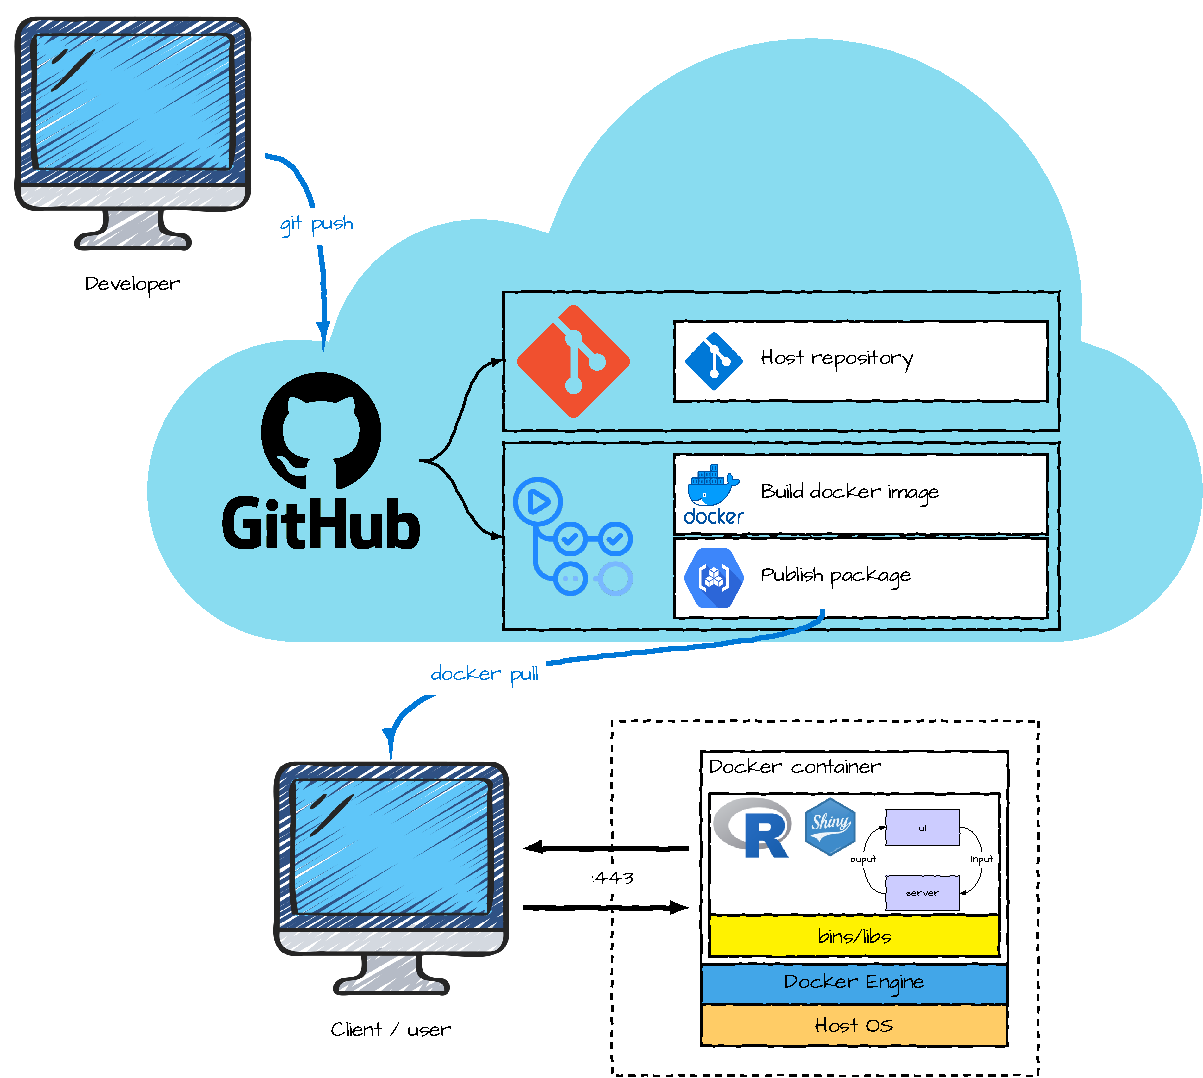
\includegraphics[keepaspectratio]{manual_files/figure-pdf/fig-diagram-1.pdf}}

}

\caption{\label{fig-diagram}Diagram illustrating the relationship
between the code produced by the developer and the shiny docker
container utilised by user with a Github cloud conduit. The developed
codebase includes a Shiny R application with R backend,
\texttt{Dockerfile} (instructions used to assemble a full operating
environment) and github workflow file (instructions for building and
packaging the docker image on github via \texttt{actions}).}

\end{figure}%

\section{Installation}\label{installation}

\subsection{Installing docker desktop}\label{installing-docker-desktop}

To retrieve and run docker containers requires the installation of
\href{https://www.docker.com/products/docker-desktop/}{Docker Desktop}
on Windows and MacOSx

\subsubsection{Windows}\label{windows}

The steps for installing Docker Desktop are:

\begin{itemize}
\item
  \textbf{Download the Installer:} head to
  \url{https://docs.docker.com/desktop/install/windows-install/} and
  follow the instructions for downloading the appropriate installer for
  your Windows version (Home or Pro).
\item
  \textbf{Run the Installer:} double-click the downloaded file and
  follow the on-screen instructions from the installation wizard. Accept
  the license agreement and choose your preferred installation location.
\item
  \textbf{Configure Resources (Optional):} Docker Desktop might suggest
  allocating some system resources like CPU and memory. These settings
  can be adjusted later, so feel free to use the defaults for now.
\item
  \textbf{Start the Docker Engine:} once installed, click the ``Start
  Docker Desktop'' button. You may see a notification in the taskbar -
  click it to confirm and allow Docker to run in the background.
\item
  \textbf{Verification:} open a terminal (or Powershell) and run
  \texttt{docker\ -\/-version}. If all went well, you should see
  information about the installed Docker Engine version.
\end{itemize}

Additional Tips:

\begin{itemize}
\tightlist
\item
  Ensure Hyper-V (virtualization) is enabled in your BIOS settings for
  optimal performance.
\end{itemize}

\subsection{Installing the and running the
app}\label{installing-the-and-running-the-app}

The task of installing and running the app is performed via a single
\textbf{deploy script} (\texttt{deploy\_wq.bat} on Windows or
\texttt{deploy\_wq.sh} on Linux/MacOSX/wsl). For this to work properly,
the deploy script should be placed in a folder along with two additional
folders (one called \texttt{input} and the other called
\texttt{parameters}) that contains the input datasets (in csv format)
and run time parameters. This structure is illustrated below for
Windows.

\begin{verbatim}
\
|- deploy_wq.bat
|- input
   |- 16_wq.csv
   |- 17_wq.csv
   |- overwrites.csv
   |- weights_m.csv
   |- weights_s.csv
|- parameters
   |- config.ini
   |- water_quality_guidelines.csv
   |- spatial.csv
   |- GIS
      |- RCZ_rev24.*
      |- SBZone_upper.*
      |- Middle_Harbour_Upper.*
\end{verbatim}

\begin{tcolorbox}[enhanced jigsaw, left=2mm, leftrule=.75mm, bottomrule=.15mm, toptitle=1mm, colbacktitle=quarto-callout-note-color!10!white, bottomtitle=1mm, arc=.35mm, colback=white, breakable, opacitybacktitle=0.6, coltitle=black, colframe=quarto-callout-note-color-frame, titlerule=0mm, toprule=.15mm, opacityback=0, title=\textcolor{quarto-callout-note-color}{\faInfo}\hspace{0.5em}{Note}, rightrule=.15mm]

In the above illustration, there are two example water quality datasets
(\texttt{16\_wq.csv} and \texttt{17\_wq.csv}). To ensure that the
application correctly identifies them as water quality datasets, it is
important that they are named according to the following format:
\texttt{\textless{}yy\textgreater{}\_wq.csv} where the
\texttt{\textless{}yy\textgreater{}} represents a two digit year
(e.g.~16 for 2016). For additional information on the contents of these
files, please see Section~\ref{sec-data-requirements}.

\end{tcolorbox}

To set up the above structure:

\begin{enumerate}
\def\labelenumi{\arabic{enumi}.}
\item
  create a new folder on your computer in a location of your choice that
  you are likely to remember and easily locate (e.g.~on the desktop).
  Whilst the name of the folder is not important, it is recommended that
  it be named after the project (e.g.
  \texttt{darwin\_harbour\_wq\_monitoring}).
\item
  download the deploy script from the projects github repository

  \begin{enumerate}
  \def\labelenumii{\alph{enumii}.}
  \item
    go to the projects github repository
    (\url{https://github.com/open-AIMS/dh_wq_monitoring.git}) in a
    browser
  \item
    click on either the \texttt{deploy\_wq.bat} (Windows) or
    \texttt{deploy\_wq.sh} (Linux/MacOSX/wsl).

    \pandocbounded{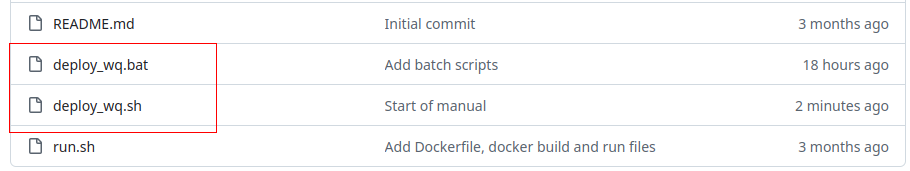
\includegraphics[keepaspectratio]{resources/github_deploy_script.png}}
  \item
    click on the download button and select the project folder as the
    location to download the file to. If the file is automatically
    downloaded to a downloads folder, move the file to the project
    folder.

    \pandocbounded{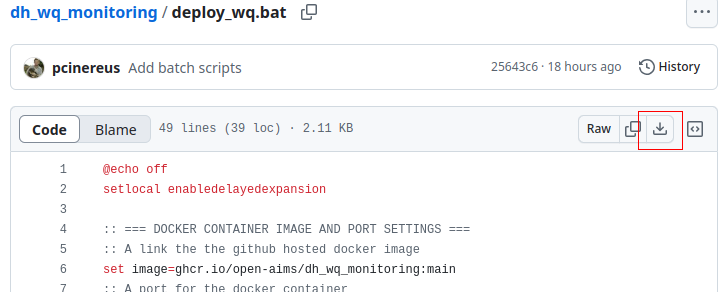
\includegraphics[keepaspectratio]{resources/github_deploy_script2.png}}
  \end{enumerate}
\item
  within the project folder, create folders called \texttt{inputs} and
  \texttt{parameters} (as outlined above) and place all the appropriate
  data sets into these folders
\end{enumerate}

To run the app, navigate inside of the project folder and run (typically
double click) on the deploy script. Upon doing so, you will be presented
with a directory selection window that is prompting for the path of the
project folder. Navigate to and select the project folder before
clicking the ``OK'' button. Shortly thereafter, the application will
appear in a browser tab.

\begin{tcolorbox}[enhanced jigsaw, left=2mm, leftrule=.75mm, bottomrule=.15mm, toptitle=1mm, colbacktitle=quarto-callout-note-color!10!white, bottomtitle=1mm, arc=.35mm, colback=white, breakable, opacitybacktitle=0.6, coltitle=black, colframe=quarto-callout-note-color-frame, titlerule=0mm, toprule=.15mm, opacityback=0, title=\textcolor{quarto-callout-note-color}{\faInfo}\hspace{0.5em}{More specific information about the \texttt{deploy\_wq.bat} script}, rightrule=.15mm]

The \texttt{deploy\_wq.bat} script performs the following:

\begin{enumerate}
\def\labelenumi{\arabic{enumi}.}
\tightlist
\item
  defines paths to the project repository and local project folder
\item
  checks if \texttt{docker} is installed and available from the command
  line for the current user
\item
  checks if \texttt{docker} is running
\item
  query the user for the location of the project folder
\item
  determine whether there are any updates to the \texttt{docker} image
  and if so pull them down
\item
  run the \texttt{docker} container
\item
  open the shiny app in a browser
\end{enumerate}

\end{tcolorbox}

\section{The Darwin Harbour Water Quality Monitoring Program Analysis
App}\label{the-darwin-harbour-water-quality-monitoring-program-analysis-app}

This \href{https://shiny.posit.co/}{Shiny} application is designed to
ingest very specifically structured water quality datasets containing
Darwin Harbour Water Quality monitoring data and produce various
analyses and visualisations. The application is served from a
\href{https://www.docker.com/}{docker} container to the localhost and
the default web browser.

Docker containers can be thought of a computers running within other
computers. More specifically, a container runs an instance of image
built using a series of specific instructions that govern the entire
software environment. As a result, containers run from the same image
will operate (virtually) identically regardless of the host environment.
Furthermore, since the build instructions can specify exact versions of
all software components, containers provide a way of maximising the
chances that an application will continue to run as designed into the
future despite changes to operating environments and dependencies.

This shiny application comprises five pages (each accessable via the
sidebar menu on the left side of the screen):

\begin{enumerate}
\def\labelenumi{\arabic{enumi}.}
\tightlist
\item
  a \textbf{Landing} page (this page) providing access to the settings
  and overall initial instructions
\item
  a \textbf{Dashboard} providing information about the progression of
  tasks in the analysis pipeline
\item
  a \textbf{Data} page providing overviews of data in various stages
\item
  a \textbf{QAQC} page providing graphical QAQC outputs
\item
  a \textbf{Summaries} page providing summaries of the bootstrap
  aggregation of indices
\item
  a \textbf{Manual} page that displays the online manual for the
  application
\end{enumerate}

Each page will also contain instructions to help guide you through using
or interpreting the information. In some cases, this will take the from
of an info box (such as the current box). In other cases, it will take
the form of little {} symbols whose content is revealed with a mouse
hover.

There are numerous stages throughout the analysis pipeline that may
require user review (for example examining any data validation issues as
well as the QAQC figures to confirm that the data are as expected).
Consequently, it is advisable for the user to manually trigger each
successive stage of the pipeline. The stages are:

\begin{itemize}
\item
  Stage 1 - Prepare environment

  More info

  This stage is run automatically on startup and essentially sets up the
  operating environment.

  \begin{itemize}
  \tightlist
  \item
    load any R package dependencies
  \item
    get runtime settings from \texttt{../params/config.ini}. These
    include:

    \begin{itemize}
    \tightlist
    \item
      \texttt{focal\_year}: usually the final year of sampling, all
      artifacts (data/graphics) will be stored in a folder reflecting
      this year
    \item
      \texttt{method}: the index method to apply when calculating
      indices
    \item
      \texttt{foldcap}: the folding cap to apply when calculating
      indices
    \item
      \texttt{tuning}: the tuning to apply when calculating indices
    \item
      \texttt{size}: the number of bootstrapp samples
    \item
      \texttt{seed}: the random seed to apply to bootstrapping
    \end{itemize}
  \end{itemize}
\item
  Stage 2 - Obtain data

  More info

  This stage comprises of the following steps:

  \begin{itemize}
  \tightlist
  \item
    read in the water quality guidelines from
    \texttt{../parameters/water\_quality\_guidelines.csv}.
  \item
    read in each of the water quality data files from
    \texttt{../input/}. These files are in the format of
    \texttt{\textless{}number\textgreater{}\_wq.csv}, where
    \texttt{\textless{}number\textgreater{}} is a two digit number
    representation of the sampling year.
  \item
    read in each of the overwrites file from
    \texttt{../input/overwrites.csv}.
  \item
    read in each of the measures weights file from
    \texttt{../input/weights\_m.csv}.
  \item
    read in each of the spatial weights file from
    \texttt{../input/weights\_s.csv}.
  \item
    read in the aggregation hierarchy file from
    \texttt{../input/hierarchy.csv}.
  \item
    read in the spatial settings file from
    \texttt{../parameters/spatial.csv}.
  \item
    validating each of the sources of input data according to a set of
    validation rules
  \end{itemize}

  The tables within the \textbf{Raw data} tab of the \textbf{Data} page
  will also be populated (but wont be available for review until after
  the data have been processed in Stage 3).
\item
  Stage 3 - Prepare spatial data

  More info

  This stage comprises of the following steps:

  \begin{itemize}
  \tightlist
  \item
    read in individual shapefiles from \texttt{../parameters/GIS}. The
    files are:

    \begin{itemize}
    \tightlist
    \item
      \texttt{RCZ\_rev24.shp}
    \item
      \texttt{SBZone\_upper.shp}
    \item
      \texttt{Middle\_Harbour\_Upper.shp}
    \end{itemize}
  \item
    combine all shapefiles into a single shapefile
  \end{itemize}

  The tables within the \textbf{Processed data} tab of the \textbf{Data}
  page will also be populated.
\item
  Stage 4 - Process data

  More info

  This stage comprises of the following steps:

  \begin{itemize}
  \tightlist
  \item
    combine all the water quality data into a single data set
  \item
    process the dates from strings into genuine date objects
  \item
    filter data to the bounds either defined in
    \texttt{../parameters/config.ini} or the data
  \item
    select only measures for which there are guideline values
  \item
    if the \texttt{focal\_year} is undefined, define it based on the
    maximum date
  \item
    pivot the data into a longer format that is more suitable for
    analysis and graphing
  \item
    join in the guidelines information
  \item
    use the spatial information in the shapefiles to assign spatial
    domains such as Regions and Zones.
  \item
    apply any unit conversions to the values
  \item
    apply limit of detection rules (to Dissolved Oxygen)
  \item
    join in the aggregation hierarchy
  \end{itemize}

  The tables within the \textbf{Processed data} tab of the \textbf{Data}
  page will also be populated and the \texttt{Data} page will be
  available for review.
\item
  Stage 5 - Calculate indices

  More info

  This stage comprises of the following steps:

  \begin{itemize}
  \tightlist
  \item
    retrieve the processed data.
  \item
    calculate the indices
  \item
    prepare for bootstrapping
  \end{itemize}
\item
  Stage 6 - QAQC

  More info

  This stage comprises of the following steps:

  \begin{itemize}
  \tightlist
  \item
    retrieve the processed data.
  \item
    construct outlier plots
  \item
    contruct an LOR table
  \item
    contruct boxplots for each Measure for the Focal Year for each Zone
  \item
    construct timeseries boxplots for each Measure/Zone
  \item
    construct boxplots for each Measure for the Focal Year conditional
    on Zone
  \end{itemize}

  The QAQC figures of the \textbf{QAQC} page will also be populated.
\item
  Stage 7 - Bootstrapping

  More info

  This stage comprises of the following steps:

  \begin{itemize}
  \tightlist
  \item
    generate bootsrapping schematic diagram
  \item
    retrieve the processed data
  \item
    retrieve the indices
  \item
    process the overwrites
  \item
    process the weights
  \item
    aggregate to Zone/Measure/Source level
  \item
    aggregate to Zone/Measure level
  \item
    aggregate to Zone/Subindicator level
  \item
    aggregate to Zone/Indicator level
  \item
    aggregate to Region/Measure level
  \item
    aggregate to Region/Subindicator level
  \item
    aggregate to Region/Indicator level
  \item
    aggregate to WH/Measure level
  \item
    aggregate to WH/Subindicator level
  \item
    aggregate to WH/Indicator level
  \end{itemize}
\item
  Stage 8 - Summaries

  More info

  This stage comprises of the following steps:

  \begin{itemize}
  \tightlist
  \item
    retrieve the processed data
  \item
    compile all the indice scores
  \item
    generate Zone/Measure/Source level
  \item
    collate Zone/Measure level scores
  \item
    collate Zone/Subindicator level scores
  \item
    collate Zone/Indicator level scores
  \item
    collate Region/Measure level scores
  \item
    collate Region/Subindicator level scores
  \item
    collate Region/Indicator level scores
  \item
    collate WH/Measure level scores
  \item
    collate WH/Subindicator level scores
  \item
    collate WH/Indicator level scores
  \item
    generate trend plots
  \item
    calculate effects (between years)
  \item
    generate effects plots
  \end{itemize}

  The trend and effects figures of the \textbf{Summaries} page will also
  be populated.
\end{itemize}

Underneath the sidebar menu there are a series of buttons that control
progression through the analysis pipeline stages. When a button is blue
(and has a play icon), it indicates that the Stage is the next Stage to
be run in the pipeline. Once a stage has run, the button will turn
green. Grey buttons are disabled.

Clicking on button will run that stage (or stages in some cases). While
the stage is in progress, a popup will be displayed over the buttons.
This popup serves two purposes. Firstly, some tasks within some stages
are computationally intense and thus take some time to perform. For such
tasks, a progress bar will be displayed in the popup to inform you of
the progress through this task. Secondly, as some stages/tasks are slow,
it provides visual feedback about when a stage has truly started and
completed and prevents the temptation to repeatedly click on a button
when nothing appears to be happening.

Once a stage is complete, the button will change to either green
(success), yellow (orange) or red (failures) indicating whether
errors/warnings were encountered or not. If the stage was completed
successfully, the button corresponding to the next available stage will
be activated.

Sidebar menu items that are in orange font are active and clicking on an
active menu item will reveal an associated page. Inactive menu items are
in grey font. Menu items will only become active once the appropriate
run stage has been met. The following table lists the events that
activate a menu item.

\begin{longtable}[]{@{}ll@{}}
\toprule\noalign{}
Menu Item & Trigger Event \\
\midrule\noalign{}
\endhead
\bottomrule\noalign{}
\endlastfoot
Landing & Always active \\
Dashboard & Always active \\
Data & After Stage 4 \\
QAQC & After Stage 6 \\
Summaries & After Stage 8 \\
Manual & Always active \\
\end{longtable}

Note, it is also possible to make all menu and buttons active using the
\textbf{Run in sequence} toggle, however this should only be used if the
full sequence of stages has already been run and you are returning to
the analyses in a later session

Figure~\ref{fig-diagram2} provides a schematic overview of the sequence
of filesystem events that occur during the development, deployment and
running of this app.

\begin{enumerate}
\def\labelenumi{\arabic{enumi}.}
\tightlist
\item
  the developed codebase is pushed to github and if necessary continuous
  integration (github actions) is triggered. The continuous integration
  will re-build and host a docker image as well as rebuild the manual.
\item
  when the client runs the \texttt{deploy\_wq.bat} (or
  \texttt{deploy\_wq.sh}) script, it will check whether docker is
  running and get input from the user about the location of the project
  directory.
\item
  github will be queried to discover if a new docker image is available.
  If so, then the new image will be pulled down locally and run (if
  docker is runnning).
\item
  the docker container will be run and this will trigger git within the
  container to pull down the latest version of the codebase from github
  to a temporary repo in the container. As the container is starting up,
  it will mount the project folder so that its contents are available to
  the environment within container and outputs produced within the
  container are available to the host.
\item
  some of the files in the temporary repo will be copied to a folder
  within the project folder.
\item
  the shiny app will start up on \texttt{port\ 3838} of the localhost
  and this will be offered to the default browser.
\item
  as the shiny app progresses through each of the analysis stages, more
  data will be added to various folders of the project directory.
\end{enumerate}

\begin{figure}

\centering{

\pandocbounded{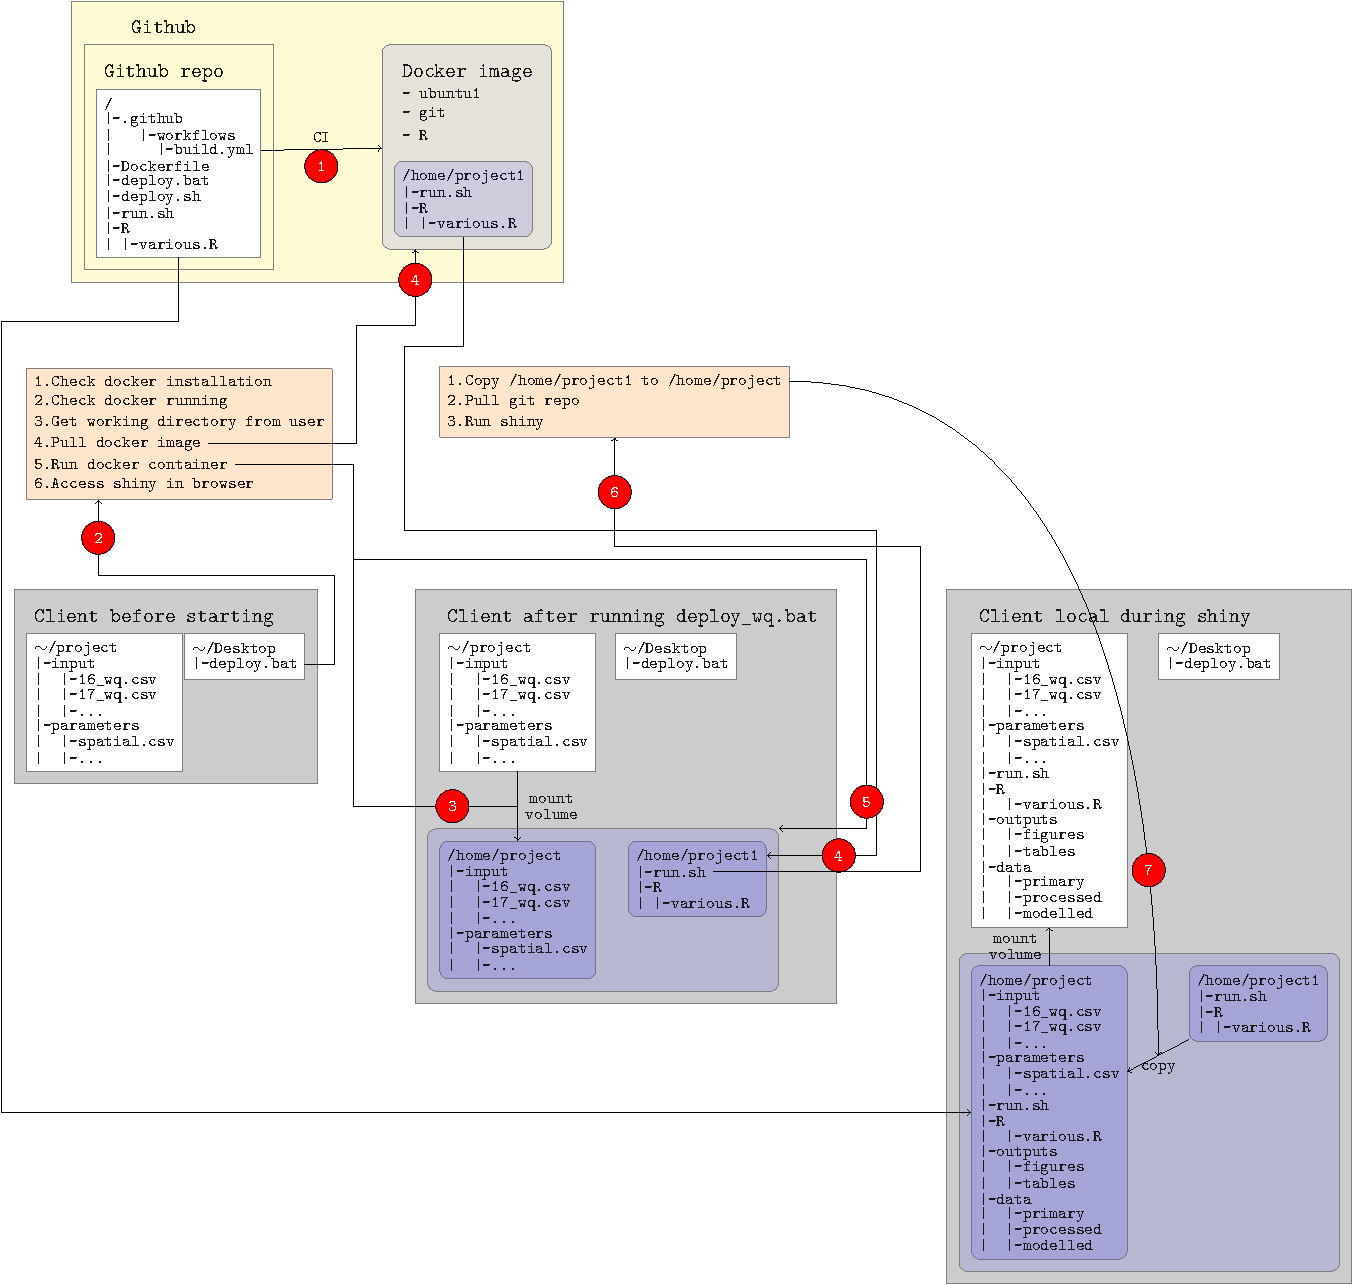
\includegraphics[keepaspectratio]{manual_files/figure-pdf/fig-diagram2-1.pdf}}

}

\caption{\label{fig-diagram2}Diagram illustrating the sequence of
filesystem events that occur during the development, deployment and
running of this app.}

\end{figure}%

\begin{tcolorbox}[enhanced jigsaw, left=2mm, leftrule=.75mm, bottomrule=.15mm, toptitle=1mm, colbacktitle=quarto-callout-note-color!10!white, bottomtitle=1mm, arc=.35mm, colback=white, breakable, opacitybacktitle=0.6, coltitle=black, colframe=quarto-callout-note-color-frame, titlerule=0mm, toprule=.15mm, opacityback=0, title=\textcolor{quarto-callout-note-color}{\faInfo}\hspace{0.5em}{Prior to starting the application}, rightrule=.15mm]

Before starting the application, it is important that you review the
following files:

\begin{itemize}
\tightlist
\item
  \texttt{../parameters/config.ini}. Specifically, review the following
  fields:

  \begin{itemize}
  \tightlist
  \item
    \texttt{focal\_year=}: indicates the year that will be considered
    the focal sampling year. All outputs will be stored in a folder
    reflecting this display diagnostics for this the focal year is the
    most recent sampling year. Furthermore, many of the QAQC diagnostics
    pertain specifically to this focal year alone.
  \item
    \texttt{method=}: indicates the index method to employ (see
    \textbf{?@sec-index-methods} for more information).
  \item
    \texttt{foldcap=}: indicates the value (on the fractional/fold
    scale) to cap indices (see \textbf{?@sec-index-foldcap} for more
    information)
  \item
    \texttt{tuning=}: indicates the tuning value used in specific index
    calculations (see \textbf{?@sec-index-tuning} for more information)
  \item
    \texttt{size=}: indicates the number of bootstrapp aggregations to
    use
  \item
    \texttt{seed}: indicates the random seed to use during any
    stoichastic process
  \item
    \texttt{start\_date}: the minimum date for analysed data. This
    allows the lower bound year of the data to be restricted (to omit
    earlier data if necessary). If this item is missing, the start\_date
    will be determined from the observed data.
  \item
    \texttt{end\_date}: the maximum date for the analysed data. This
    allows the upper bound year of the data to be restricted (to omit
    later data if necessary). If this item is missing, the end\_date
    will be determined from the observed data.
  \end{itemize}
\item
  \texttt{../parameters/water\_quality\_guidelines.csv}. This file
  defines the guideline values associated with each measure as well as
  the labels to be used in tables/figures.
\item
  \texttt{../parameters/spatial.csv}. This file defines the names used
  for Zones and Areas.
\item
  \texttt{../input/overwrites.csv}. This file defines any expert
  overwrites that should be applied (in the event that the observed
  values are considered unrepresentative or unsuitable for some
  justifiable reason).
\item
  \texttt{../input/weights\_m.csv}. This file provides any specific
  weights that should be applied when aggregating items together on the
  Measure scale.
\item
  \texttt{../input/weights\_s.csv}. This file provides any specific
  weights that should be applied when aggregating items together on the
  spatial scale.
\end{itemize}

\end{tcolorbox}

\section{Analyses}\label{analyses}

Before describing the sequence of steps in the analysis pipeline, it is
necessary to outline the major conceptual phases of the analyses.

\subsection{Index computation}\label{sec-index-computation}

Water Quality indices (which are standardized measures of condition) are
typically expressed relative to a guideline (see Appendix
(\textbf{sec:guidelines?}) on page (\textbf{sec:guidelines?})) or
benchmark. Of the numerous calculation methods available, those that
take into account the distance from the guideline (i.e.~incorporate
\emph{difference-to-reference}) rather than simply an indication of
whether or not a guideline value has been exceeded are likely to retain
more information as well as being less sensitive to small changes in
condition close to the guidelines.

The challenging aspect of distance (or amplitude) based index
methodologies is that what constitutes a large deviation from a
benchmark depends on the scale of the measure. For example, a deviation
of 10 units might be considered relatively large of turbidity (NTU) or
salinity (ppt), yet might be considered only minor for the Total
Nitrogen (\(\mu g/L\)). In order to combine a range of such metrics
together into a meaningful index, the individual scores must be
expressed on a common scale. Whilst this is automatically the case for
Binary compliance, it is not necessarily the case for distance based
indices.

Table~\ref{tbl-indexMethods} describes and compares the formulations and
response curves of the Binary compliance method as well as a number of
amplitude (distance based) indexing methods.

The Modified Amplitude and Logistic Modified Amplitude are both based on
a base 2 logarithm of the ratio of observed values to the associated be
benchmark (see Table~\ref{tbl-indexMethods}). This scale ensures that
distances to the benchmark are symmetric (in that a doubling and halving
equate to the same magnitude - yet apposing sign). Furthermore, the
logarithmic transformation does provide some inbuilt capacity to
accommodate log-normality (a common property of measured values).

By altering the sign of the exponent, the Modified Amplitude methods can
facilitate stressors and responses for which a failure to comply with a
benchmark would be either above or below the benchmark (e.g. NTU vs
Secchi depth). Further modifications can be applied to accommodate
measures in which the benchmark represents the ideal and deviations
either above or below represent increasingly poorer conditions (e.g.~pH
and dissolved oxygen).

The raw Modified Amplitude scores are relatively insensitive to small
fluctuations around a benchmarks and sensitivity increases exponentially
with increasing distance to the benchmark. The resulting scores can take
any value in the real line {[}\(-\infty, \infty\){]} and hence are not
bounded\textbackslash footnote\{Unbounded indices are difficult to
aggregate, since items that have very large magnitude scores will have
more influence on the aggregation than those items with scores of
smaller magnitude. Furthermore, unbounded scores are difficult to
convert into alphanumeric Grades. Consequently, the Scores need to be
scaled before they can be converted to alphabetical grading scale. There
are two broad approaches to scaling (see Table~\ref{tbl-indexMethods}):

\begin{enumerate}
\def\labelenumi{\alph{enumi}.}
\item
  Capping and scaling: The \(log_2\) scale can be capped to a range
  representing either a constant extent of change (e.g.~twice and half
  the benchmark - a cap factor of 2) or else use historical quantiles
  (10th and 90th percentiles) to define the upper and lower bounds to
  which to cap the scale. Note historical quantiles are unavailable for
  the current application. Thereafter, either can be scaled to the range
  {[}0,1{]} via a simple formula (see Table~\ref{tbl-indexMethods}
  III.Scaled).
\item
  Logistic Modified Amplitude: By expressing the scores on a logistic
  scale, the range of scores can be automatically scaled to range
  {[}0,1{]}. Moreover, this method allows the shape of the response
  curve to be customized for purpose. For example, the relative
  sensitivity to changes close or far from the benchmarks can be altered
  by a tuning parameter.
\end{enumerate}

Rather than aggregating across sites before calculating indices, we
would suggest that indices should be calculated at the site level. This
is particularly important when different measures are measured at
different sites. Spatial variability can be addressed via the use of a
bootstrapping routine (see below). We would recommend that measurements
collected throughout the reporting year be aggregated together into a
single annual value. This is primarily because most water quality
guidelines pertain specifically to annual averages rather than single
time samples. Although it is possible to incorporate uncertainty due to
temporal variability, the low sparse temporal frequency of sample
collection is likely to yield uncertainty characteristics that will
swamp the more interesting spatial sources of uncertainty.

A useful metric for comparing the sensitivity of one indexing method
over another is to take some representative longitudinal data and
calculate indices based on the actual data as well as data that
introduces progressively more noise.

In the absence of longitudinal data, it is possible to compare final
outcomes based on each indexing formulation. Appendix
\ref{sec:indexMethods} on \pageref{sec:indexMethods} provides
comparisons of three index formulations (Binary, fsMAMP: Fixed cap
Scaled Modified Amplitude and lMAMP: Logistic Modified Amplitude) for a
range of spatial and Measurement hierarchical levels. It is not possible
to offer quantile based scaling for the Modified Amplitude methods as
long-term quantiles associated with the guideline values are not
available.

\begin{longtable}[]{@{}
  >{\raggedright\arraybackslash}p{(\linewidth - 4\tabcolsep) * \real{0.1000}}
  >{\raggedright\arraybackslash}p{(\linewidth - 4\tabcolsep) * \real{0.7800}}
  >{\raggedright\arraybackslash}p{(\linewidth - 4\tabcolsep) * \real{0.1200}}@{}}

\caption{\label{tbl-indexMethods}Formulations and example response
curves for a variety of indicator scoring methods that compare observed
values (\(x_i\)) to associated benchmark, guidelines or references
values (\(benchmark_i\) and dashed line). The Scaled Modified Amplitude
Method can be viewed as three Steps: I. Initial Score generation, II.
Score capping (two alternatives are provided) and III. Scaling to the
range {[}0,1{]}. The first of the alternative capping formulations
simply caps the Scores to set values (on a \(log_2\) scale), whereas the
second formulation (Quantile based, where \(Q1\) and \(Q2\) are
quantiles) allows guideline quantiles to be used for capping purposes.
Dotted lines represent capping boundaries. In the Logistic Scaled
Amplitude method, \(T\) is a tuning parameter that controls the logistic
rate (steepness at the inflection point). For the purpose of example,
the benchmark was set to 50.}

\tabularnewline

\toprule\noalign{}
\begin{minipage}[b]{\linewidth}\raggedright
Method
\end{minipage} & \begin{minipage}[b]{\linewidth}\raggedright
Formulation
\end{minipage} & \begin{minipage}[b]{\linewidth}\raggedright
Response curve
\end{minipage} \\
\midrule\noalign{}
\endhead
\bottomrule\noalign{}
\endlastfoot
Binary & \(
score_i = \left\{ 
\begin{array}{l l}
1 & \text{if}~x_i \le benchmark_i\\
0 & \text{if}~x_i~\text{else}\\
\end{array}
\right.
\) &
\pandocbounded{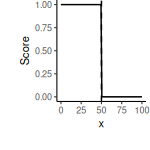
\includegraphics[keepaspectratio]{manual_files/figure-pdf/binary.png}} \\
Benchmark and WCS & \(
score_i = \left\{ 
\begin{array}{l l}
100 & \text{if}~x_i \le benchmark_i\\
0 & \text{if}~x_i~\ge WCS_i\\
\left[1.0 - \lvert\frac{x_i - benchmark_i}{WCS_i - benchmark_i}\lvert\right].100 & \text{else}\\
\end{array}
\right.
\) &
\pandocbounded{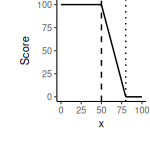
\includegraphics[keepaspectratio]{manual_files/figure-pdf/wcs.png}} \\
Modified Amplitude & & \\
I. Raw (MAMP) & \(
score_i = \left\{ 
\begin{array}{l l}
log_2(\frac{x_i}{benchmark_i})^{-1} & \text{if}>benchmark_i=\text{fail}\\
log_2(\frac{x_i}{benchmark_i})^{1} & \text{if}<benchmark_i=\text{fail}\\
\end{array}
\right.
\) &
\pandocbounded{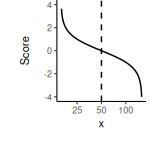
\includegraphics[keepaspectratio]{manual_files/figure-pdf/mamp.png}} \\
II. Fixed caps (-1, 1) & \(
Score_i = \left\{
\begin{array}{l l}
log_2(-1) & \text{if}~Score_i < -1\\
log_2(1) & \text{if}~Score_i > 1\\
Score_i &otherwise\\
\end{array}
\right.
\) &
\pandocbounded{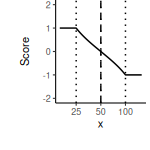
\includegraphics[keepaspectratio]{manual_files/figure-pdf/cmamp.png}} \\
II. Quantile based caps & \(
Score_i = \left\{
\begin{array}{l l}
log_2(\frac{Q1}{benchmark_i})^{-1} & \text{if}~x_i<Q1\\
log_2(\frac{Q2}{benchmark_i})^{1} & \text{if}~x_i>Q2\\
Score_i &otherwise\\
\end{array}
\right.
\) &
\pandocbounded{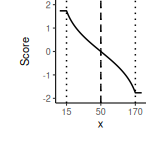
\includegraphics[keepaspectratio]{manual_files/figure-pdf/qmamp.png}} \\
III. Scaled & \(
Score_i = \frac{Score_i - min(Score_i)}{max(Score_i) - min(Score_i)}
\) &
\pandocbounded{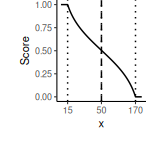
\includegraphics[keepaspectratio]{manual_files/figure-pdf/smamp.png}} \\
Logistic Scaled Modified Amplitude & \(
\lambda_i = 
\begin{cases} -1 & \text{if}>benchmark_i=\text{fail}\\
1 & \text{if}<benchmark_i=\text{fail}
\end{cases};
R_i =
\begin{cases} -1 & \text{if}>benchmark_i=\text{fail}\\
1 & \text{if}<benchmark_i=\text{fail}
\end{cases};\newline
Score_i=\frac{1}{1+e^{\lambda R_i T}}
\) &
\pandocbounded{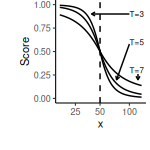
\includegraphics[keepaspectratio]{manual_files/figure-pdf/logistic.png}} \\

\end{longtable}

\subsection{Bootstrapping}\label{bootstrapping}

Bootstrapping is a statistical resampling method that involves
repeatedly sampling with replacement from a dataset to estimate the
sampling distribution of a statistic. By generating multiple ``bootstrap
samples,'' this technique allows for the computation of measures such as
confidence intervals, standard errors, and other uncertainty metrics
without relying on strong parametric assumptions.

Bootstrapping is particularly useful for aggregating collections of data
while retaining the combined uncertainty through the aggregation
process. When data from multiple sources or experiments are combined,
the uncertainty associated with each dataset must be accounted for to
avoid underestimating the variability in the aggregated result.
Bootstrapping achieves this by:

\begin{itemize}
\tightlist
\item
  \emph{Resampling with replacement}: This ensures that the variability
  within each dataset is preserved and propagated into the aggregated
  result.
\item
  \emph{Estimating uncertainty}: By calculating statistics (e.g., means,
  medians, or other metrics) across bootstrap samples, bootstrapping
  provides a robust way to quantify the uncertainty in the aggregated
  data.
\item
  \emph{Non-parametric flexibility}: Bootstrapping does not require
  assumptions about the underlying distribution of the data, making it
  suitable for complex or non-standard datasets.
\end{itemize}

In summary, bootstrapping is a powerful tool for combining data while
retaining all sources of uncertainty, ensuring that the aggregated
results accurately reflect the variability inherent in the original
datasets.

\subsection{Hierarchical aggregation}\label{sec-hierAgg}

To facilitate the integration of additional input Measures into the
report card scores (such as additional Physico-chem or nutrients), or
even additional Sub-indicators (such as sediment metals, seagrasses and
mangroves), we can defined a hierarchical structure in which Measures
(such as Turbidity, NOx, etc) are nested within appropriate
Sub-indicators. In turn, these Sub-indicators are nested within
Indicators.

By progressively abstracting away the details of the Measures and
Sub-indicators, a more focused narrative can be formulated around each
level of the hierarchy. For example, when discussing the current state
(and trend in state) of the Water Quality Indicator, rather than needing
to discuss each individual constituent of Water Quality, high-level
Grades are available on which to base high-level interpretations. More
detailed explorations are thence revealed as required by exploring the
Grades at progressively finer scales of the hierarchy. Moreover, the
hierarchical structure offers great redundancy and thus flexibility to
add, remove and exchange individual measures.

Similar arguments can be made for a spatial hierarchy in which Zones are
nested within Regions which in turn are nested within the Whole Harbour.

The current hierarchical structure comprises two physico-chemical
Measures (Dissolved Oxygen and Turbidity) that are nested within a
single Physico-chem Sub-indicator and four nutrient Measures (Ammonia,
Chlorophyll-a, Filterable Reactive Phosphate and NOx) that are nested
within a single Nutrient Sub-indicator.

There is future scope to add additional nutrient or physico-chemical
Measures as well as metals and sediments. This hierarchy can be extended
down to include other environmental indicators pertaining to habitats
(mangroves, seagrass, corals) or other perspectives (cultural and
economic).

The purpose of aggregation is to combine together multiple items of
data. The current proposed Darwin Harbour report card is informed by a
double hierarchical data structure in which Measures are nested within
Sub-indicators which are nested in Indicators and Zones are nested
within Regions which are nested within Whole of Harbour (see
Figure~\ref{fig-hierarchies}).

\begin{figure}

\centering{

\pandocbounded{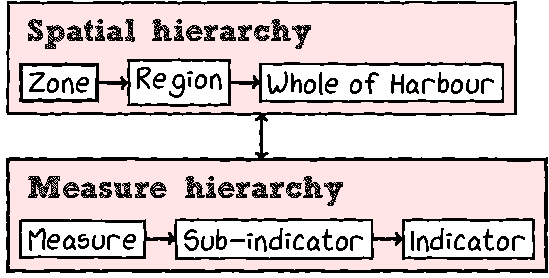
\includegraphics[keepaspectratio]{manual_files/figure-pdf/fig-hierarchies-1.pdf}}

}

\caption{\label{fig-hierarchies}Schematic illustrating the Spatial and
Measure aggregation hierarchies.}

\end{figure}%

Although the double hierarchy (Spatial and Measurement), does offer
substantial redundancy and power advantages, it also introduce the
complexity of how to combine the hierarchies into a single hierarchical
aggregation schedule. Table~\ref{tbl-complexity} (a fabricated example),
illustrates this complexity for aggregating across Spatial and Measure
scales when data availability differs. This simple example demonstrates
how different aggregation schedules can result in different Whole of
Harbour Component Scores:

\begin{itemize}
\tightlist
\item
  calculating Whole of Harbour Component Score as the average of the
  Region level Water Quality Scores prioritizes that the Whole of
  Harbour Component Score should reflect the average of the Water
  Quality Indicator Scores for the Regions. This schedule will bias the
  resulting Whole of Harbour Water Quality Indicator Score towards
  Sub-indicators represented in more Regions. Although the entire Darwin
  Harbour sampling design is currently balanced, there is no guarantee
  that this will always be the case. If for example, Nutrients were not
  available for certain Regions, then the Whole of Harbour Indicator
  Score will be biased towards Physico-chemical Sub-indicators.
\item
  calculating Whole of Harbour Water Quality Indicator Score as the
  average of the Whole of Harbour level Sub-indicator Scores prioritizes
  equal contributions of Sub-indicators to the Indicator Score at the
  expense of being able to relate Whole of Harbour Scores to the
  corresponding Region Scores.
\end{itemize}

\begin{table}

\caption{\label{tbl-complexity}Fabricated illustration of the
discrepancies between total means (i.e.~Whole of Harbour Indicator
Score) generated from row means (Region Sub-indicator Scores) and column
means (Whole of Harbour Sub-indicator Scores).}

\centering{

\begin{tabular}[t]{l|l|l|l}
\hline
\multicolumn{1}{c|}{ } & \multicolumn{2}{c|}{Sub-Indicators} & \multicolumn{1}{c}{ } \\
\cline{2-3}
Region & Physico - chem & Nutrients & Indicator\\
\hline
1 & 5.00 & 2 & 3.50\\
\hline
2 & 6.00 &  & 6.00\\
\hline
3 & 6.00 & 4 & 5.00\\
\hline
Whole of Harbour & 5.67 & 3 & X\\
\hline
\end{tabular}

}

\end{table}%

If X (mean) is calculated from the three row means = 4.83, If X (mean)
is calculated from the two column means = 4.33

Figure~\ref{fig-hier} illustrates the proposed aggregation schedule for
Darwin Report Cards. Importantly, all \emph{Indicator} Scores are
generated from \emph{Zone} level data and separate \emph{Zone} and
\emph{Whole of Harbour} level Measure aggregations are maintained in
parallel starting at the level of \emph{Indicator}.

\begin{figure}

\centering{

\pandocbounded{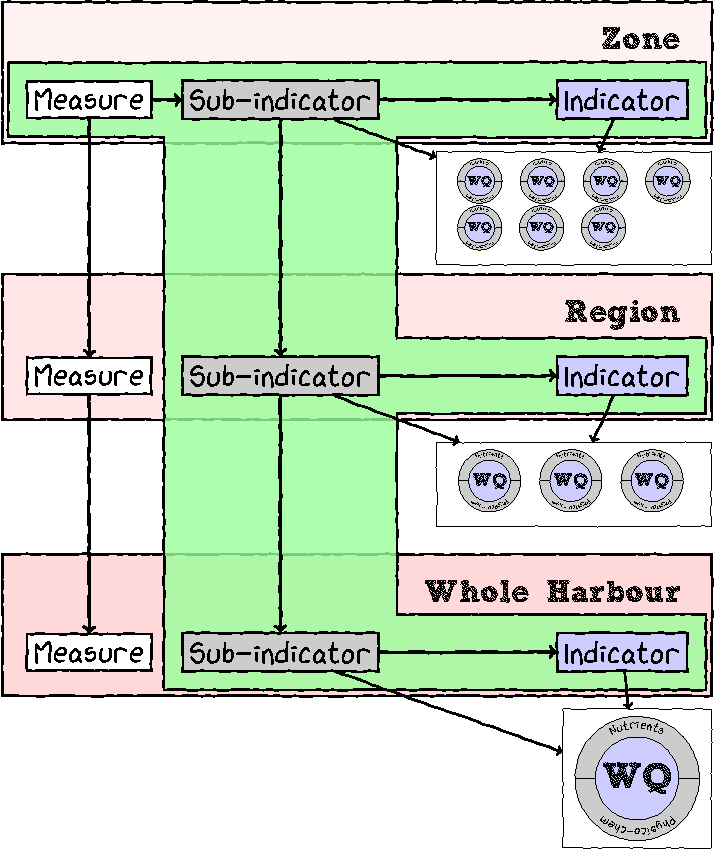
\includegraphics[keepaspectratio]{manual_files/figure-pdf/fig-hier-1.pdf}}

}

\caption{\label{fig-hier}Schematic illustrating the combination of
Spatial (Zone, Region and Whole of Harbour) and Measure (Measure,
Sub-indicator, Indicator) nodes of the double hierarchical aggregation
schedule associated with the Darwin Harbour Report Card. Aggregation
directions between nodes are signified by arrows and the main
aggregation pathway through the schedule is illustrated by the green
polygon. Tabular summaries are produced at each node, and Water Quality
Status discs (comprising Sub-indicators around a central Indicator Grade
indicate where in the hierarchy they are generated.}

\end{figure}%

Important notes on this aggregation schedule:

\begin{itemize}
\tightlist
\item
  Water Quality Indicator Scores (and thus Grades) should be the
  aggregate of the constituent Sub-indicator Scores for the appropriate
  spatial scale and thus, both derived directly from Sub-indicator level
  data.
\item
  Sub-indicator and Indicator level data often comprise data from
  differing numbers of Zones. To avoid biases towards Indicators from
  more Zones, Region and Whole of Harbour Indicator Scores should be
  calculated from Region and Whole of Harbour Indicator level data
  respectively.
\item
  That is, Whole or Harbour Indicator Scores should not be calculated
  from Region Indicator Scores.
\item
  As such, at the Indicator level Whole of Harbour Scores cannot be
  viewed as the average of the Region level Indicator data as they are
  both based on Sub-indicator data from different spatial scales
  (Regions vs Whole of Harbour).
\item
  Consequently, Sub-indicator level data are the transferable level data
  through the spatial hierarchy.
\item
  Region and Whole of Harbour Measure level data can be derived by
  aggregating down the spatial hierarchy, yet these are end of line
  derivatives that do not inform their respective Sub-indicator level
  data.
\end{itemize}

To maximize information retention throughout a series of aggregations,
it is preferable to aggregate distributions rather than single
properties of those distributions (such as means). The simplest way to
perform a hierarchy of aggregations is to interactively calculate the
means (or median) of items (means of means etc). At each successive
aggregation level only very basic distributional summaries (such as the
mean and perhaps standard deviation) are retained, the bulk of upstream
information is lost. Alternatively, more complex methods that involve
combining data or probability distributions can be effective at
aggregating data in a way that propagates rich distributional properties
throughout a series of aggregations.

Importantly, if the purpose of aggregation is purely to establish a new
point estimate of the combined items, a large variety of methods
essentially yield the same outcomes. On the other hand, if the purpose
of aggregation is also to propagate a measure of uncertainty or
confidence in the point estimate through multiple hierarchical levels of
aggregation (as is the case here), then the different methodologies
offer differing degrees of flexibility and suitability.

Hierarchical aggregations are essentially a series of steps that
sequentially combine distributions (which progressively become more data
rich). The resulting distribution formed at each step should thereby
reflect the general conditions typified by its parent distributions and
by extension, each of the distributions higher up the hierarchy.

Numerous characteristics can be estimated from a distribution including
the location (such as mean and median) and scale (such as variance and
range). For the current project, the mean and variance were considered
the most appropriate\footnote{The aggregations
typically involve some Measures with a small number of unique
observations (and thus indices) and thus means and variances provide
greater sensitivity than medians and ranges. Moreover, the indexing
stage effectively removes outliers and standardizes the scale range
thereby reducing the need for robust estimators.} distributional
descriptions and from these estimates Grades and measures of confidence
can be respectively derived. Hence the numerical summaries (mean and
variance) at any stage of the hierarchical aggregation are a byproduct
rather than the sole property of propagation.

\subsection{Bootstrap aggregation}\label{bootstrap-aggregation}

Although some of the items to be aggregated together might initially
comprise only a few values (or even a single value), it is useful to
conceptualize them as continuous distributions. For example, when
aggregating multiple \emph{Measures} (such as all Water Quality Metals)
together to generate a \emph{Site} level) \_Sub\_indicator average, each
\emph{Measure} in each \emph{Site} can be considered a distribution
comprising the single Score for that \emph{Measure}. Aggregation then
involves combining together the multiple distributions into a single
amalgam (by adding the distributions together, see Figure
Figure~\ref{fig-bootstrap}). Similarly, when aggregating at the
\emph{Indicator} level across \emph{Site} to generate \emph{Zone}
summaries for each \emph{Indicator}, \emph{Site} distributions are
respectively added together to yield a single distribution per
\emph{Zone}.

\begin{figure}

\centering{

\pandocbounded{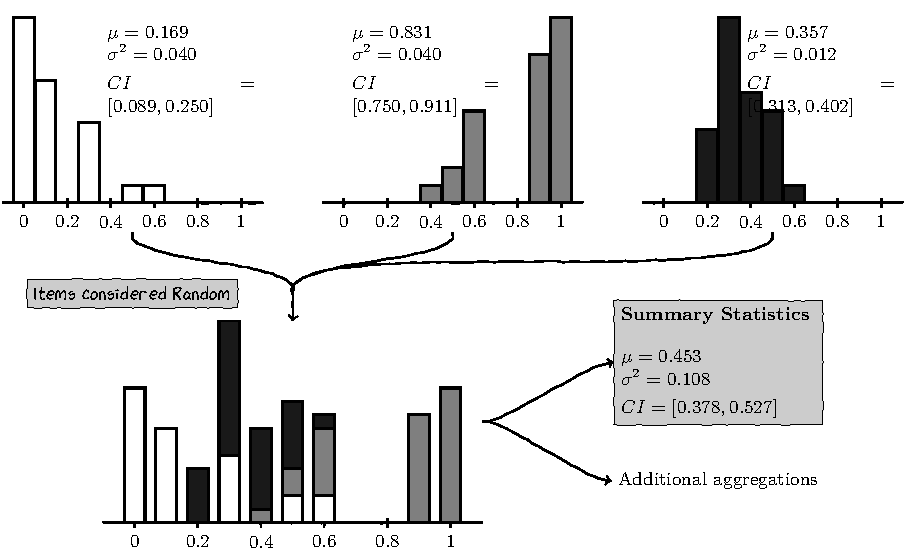
\includegraphics[keepaspectratio]{manual_files/figure-pdf/fig-bootstrap-1.pdf}}

}

\caption{\label{fig-bootstrap}Illustration of Bootstrapped aggregation
of three distributions. Simple summary statistics (mean, variance and
95\% confidence interval presented for each distribution.}

\end{figure}%

If the distributions being aggregated are all proportional distributions
(e.g.\textasciitilde density distributions), adding them altogether is
trivially simple. However, if, rather than actual distributions, the
items to be aggregated are actually just small collections of values (as
is the case for many of the measures here) or even large, yet unequally
populous collections of values (as could be the case for Continuous Flow
Monitoring with missing or suspect observations), then simply
aggregating the distributions together will result in amalgams that are
weighted according to the size of the collections (larger collections
will have more influence). For example, if we were aggregating together
three \emph{Regional} (to yield Whole of Harbour estimates), one of
which comprised twice as many Zones, simple aggregation of distributions
would result in a distribution that was more highly influenced by the
Region with the more \emph{Zones}. Similarly, when aggregating from the
level of Sub-indicator to the level of Indicator, the resulting
Indicator would be biased towards the Sub-indicator with the most
Measures. Whilst this may well be a useful property
(e.g.\textasciitilde stratified aggregation), it may also be
undesirable.

Bootstrapping is a simulation process that involves repeated sampling
(in this case with replacement) of a sample set with the aim of
generating a bootstrap sample from a distribution. This bootstrap sample
can be used to estimate the underlying probability distribution function
that generated the data as well as any other summary statistics.
Importantly, bootstrapping provides a way to generate distributions that
are proportional and thus un-weighted by the original sample sizes
thereby facilitating un-weighted aggregation. Bootstrapped distributions
can be aggregated (added together) to yield accumulated child
distributions that retain the combined properties of both parents (see
Figure~\ref{fig-bootstrap}). As a stochastic process, repeated
calculations will yield slightly different outcomes. Nevertheless, the
more bootstrap samples are collected, the greater the bootstrap
distributions will reflect the underlying Score distribution and
provided the number of drawn samples is sufficiently large (e.g.~10,000
re-samples), repeated outcomes will converge.

\subsection{Weights}\label{weights}

Standard bootstrapping yields equally weighted distributions, however,
specific weighting schemes can also be easily applied by bootstrapping
in proportion to the weights. For example, to weight one parent twice as
high as another, simply collect twice as many re-samples from the first
distribution. To ensure that all resulting distributions have the same
size (by default 10,000 items), the number of bootstrap samples
collected (\(n\)) from each of the (\(p\)) parent distributions (\(i\)),
given the weights (\(w_i\)) is calculated as:

\[
n_i = \lceil(S/p)\times w_i \rceil
\]

where \(S\) is the target size (10,000) and \(\lceil.\rceil\) indicates
the ceiling. Qualitative data (such as ratings) can also be incorporated
by enumerating the categories before bootstrapping.

In addition to allowing expert driven weights that govern the
contribution of different items during aggregations, it is possible to
weight according to relative spatial areas during spatial aggregations.
Currently, all Zones are equally weighted when aggregating to Region
level and all Regions equal when aggregating to Whole of Harbour level.
That means that small Zones have an equal contribution as large Zones
despite representing a smaller fraction of the water body. Area based
weights could be applied such that Zones and Regions contribute in
proportion to relative areas.

Weights are defined by a user editable configuration file that is
similar in structure to the Water Quality guidelines file.

\subsection{Expert interventions}\label{expert-interventions}

The ability for experts and Report Card managers to intervene (exclude
or overwrite) Scores/Grades at any Spatial/Measure scale is essential to
maintain the quality of a Report Card in the event of unrepresentative
or suspect data. The current system is able to support expert
interventions in the form of exclusions and overwrites. For example,
after reviewing the QAQC, an expert can elect to exclude one or more
Measures (or Subindicators etc) from one or more spatial scales. Such
interventions are specified via a user editable configuration
files\footnote{Since aggregation occurs across two
hierarchies (the Measure hierarchy and the Spatial hierarchy - see
@fig-hierarchies and @fig-hier), two configuration files are
necessary.} (csv) that is similar in structure to the Water Quality
guidelines file.

The essential component of this configuration file is that it allows a
user to specify what Data are to be excluded or replaced. These can be
at any of the levels of the Measure hierarchy (Measures, Sub-indications
and Indicators) and any level of the Spatial hierarchy (Zones, Regions
and Whole of Harbour). Settings pertaining to levels further along the
aggregation hierarchies have precedence. For example, if Nutrients are
excluded (or overridden) in a particular Region, then all Nutrient
Measures within all Zones will be excluded irrespective of what the
settings are for any specific Measure/Zone.

To reiterate, the advantage of bootstrapping data before concatenating
(or averaging) versus simply concatenating data from multiple sources
together, is to ensure that source data are all of exactly the same
sample size (so as to not weight more heavily towards the more populous
source(s)\footnote{Such weightings should be handled in other
ways if at all}). Bootstrapping also provides a mechanism for
propagating all distribution information throughout an aggregation
hierarchy and ensures that estimates of variance derived from child
distributions are on a consistent scale\footnote{Variance is inversely
proportional to sample size}. The latter point is absolutely critical if
variance is going to be used to inform a Confidence Rating system and
confidence intervals.

Minimum operator procedures are supported by filtering on the lowest
performed indicator prior to bootstrapping. Importantly, the
bootstrapping routine simply provides a mechanism to collate all sources
together to yield a super distribution. Thereafter, the joint
distribution can be summarized in what ever manner is deemed appropriate
(arithmetic, geometric, harmonic means, medians, variance, range,
quantiles etc). Moreover, different levels of the aggregation can be
summarized with different statistics if appropriate.

\subsubsection{Scores and Grades}\label{scores-and-grades}

The double hierarchy Bootstrap aggregation described above, yields
\emph{Score} distributions for each Measure-level/Spatial-level
combination. The location and scale of each distribution can thus be
described by its mean and variance. Mean \emph{Score} are then converted
into a simple five-point alphanumeric \emph{Grade} scale (and associated
colors) using a control chart (see Table (\textbf{tab-control?})).

\begin{longtable}[]{@{}lll@{}}
\caption{Darwin Harbour Report Card Grade scale control
chart.}\tabularnewline
\toprule\noalign{}
Score & Grade & Description \\
\midrule\noalign{}
\endfirsthead
\toprule\noalign{}
Score & Grade & Description \\
\midrule\noalign{}
\endhead
\bottomrule\noalign{}
\endlastfoot
\(\ge 0.85\) & A & Very good \\
\(\ge 0.65, <0.85\) & B & Good \\
\(\ge 0.5, <0.65\) & C & Satisfactory \\
\(\ge 0.25, <0.5\) & D & Poor \\
\(<0.25\) & E & Very poor \\
\end{longtable}

The control chart grade boundaries adopted for the current report
(presented in (\textbf{tab-control?})) are consistent with the Gladstone
Healthy Harbour Partnership Report Card. Broadly, they represent two
levels (Poor and Very Poor) under the Guideline values and three above
(Satisfactory, Good and Very Good). The grade boundaries are usually
determined by expert panel to ensure that the range of indices
represented by each grade classification is congruent with community
interpretation of a letter grade report cards. It is far less clear how
estimates of uncertainty can be incorporated into such a grading scheme
in a manner that will be intuitive to non-technical audiences. That
said, statistical uncertainty is just one of many sources of un-
certainty that should be captured into a confidence or certainty rating.
Hence any expectations of presenting uncertainty in a quantitative
manner may well be unrealistic anyway.

\subsubsection{Certainty rating}\label{certainty-rating}

Incorporating an estimate of scale (variance) into a certainty or
confidence rating necessitates re-scaling the estimates into a standard
scale. In particular, whereas a scale parameter of high magnitude
indicates lower degrees of certainty, for a certainty rating to be
useful for end users, larger numbers should probably represent higher
degrees of certainty. Thus, the scaling process should also reverse the
scale. Furthermore, variance is dependent on the magnitude of the
values.

In order to re-scale a scale estimate into a certainty rating, it is
necessary to establish the range of values possible for the scale
estimate. Whilst the minimum is simple enough (it will typically be 0),
determining the maximum is a little more challenging depending on the
aggregation algorithm (bootstrapping, Bayesian Network etc). One of the
advantages in utilizing proportional distributions (such as is the case
for a Bayesian Network or a re-sampled bootstrap distribution) is that
the scale parameter for the single worst case scenario can be devised
(once the worst case scenario has been determined) independent of sample
sizes or weightings. In most situations this is going to be when the
distribution comprises equal mass at (and only at) each of the two
extremes (for example, values of just 0 and 1).

The measure of confidence rating discussed above is purely an objective
metric derived from the variance in the aggregation hierarchy. It is
completely naive to issues such as missing data, outliers and Limit of
Detection issues - the influences of which on a confidence rating are
necessarily subjective. A full Confidence Rating would combine these
objective variance component with additional subjective considerations
such as climatic and disturbance information, and the perceived
influence of missing, Limit of Detection and outlying data. Hence, the
statistical scaled statistical variance would form just one component in
the Confidence Rating system.

The bootstrap aggregation method provides a mechanism for estimating
variance from which to build such an expert considered Confidence Rating
system.

\subsubsection{Confidence intervals}\label{confidence-intervals}

Confidence intervals (CI) represent the intervals in which we have a
certain degree of confidence (e.g.~95\%) that repeated estimates will
fall. Hence the 95\% CI of the mean is the range defined by the
quantiles representing 95\% of repeated estimates of the mean.

To calculate 95\% confidence intervals for bootstrap aggregated
distributions (e.g.~Zone 1/Nutrient distribution), we
repeatedly\footnote{The more repeated draws the closer the
distribution of means will converge. For the current project, the
number of repeated draws is 10,000.} draw a single sample from each of
the constituent distributions (e.g.~a single value from the Zone 1
Ammonia, Chlorophyll-a, Filterable Reactive Phosphate and NOx
distributions) and from each set of draws, calculate the weighted
\footnote{Weights according to the weights defined for that level of
the aggregation hierarchy} mean of the values. The 95\% CI is thus
calculated as the quantiles (p=0.025 and p=0.975) of the means.

\subsection{Aggregation schedule}\label{aggregation-schedule}

A. Calculation of Zone level Scores and Grades

\begin{enumerate}
\def\labelenumi{\arabic{enumi}.}
\item
  Collect raw data (= \textbf{Measures}) at each fixed monitoring site
  or along a Continuous Flow Monitoring (CFM) transect and compare
  individual observations to associated guideline/benchmark/reference
\item
  Create indexed data as an expression of degree of difference
  \emph{scaled modified amplitude method}) to yield a \textbf{Score} for
  each \textbf{Measure} per sampling location (e.g.~site or location
  along CFM transect) (applies to \emph{Measures} in all
  \emph{Indicators}, Water Quality)
\item
  Apply any expert opinion interventions
\item
  Combine \textbf{Measure} Scores into \textbf{Zone}-level
  \textbf{Sub-indicator} Scores by averaging taking into account any
  weightings, i.e. aggregate into observation-level Sub-indicator
  Scores. This step involves \textbf{Bootstrapping} each input to
  distributions of 10,000 re-samples (or fewer if weighted), combining
  distributions and finally Bootstrapping again into a single 10,000
  size distribution.
\item
  Combine \textbf{Sub-indicator} Scores into \textbf{Zone}-level
  \textbf{Indicator} Scores by averaging, i.e.~aggregate into Zone-level
  Indicator Scores.
\item
  Convert Scores into coloured \textbf{Grades} (A-E) for visual
  presentation in report card
\end{enumerate}

B. Calculation of Region level Grades

\begin{enumerate}
\def\labelenumi{\arabic{enumi}.}
\item
  Aggregate \textbf{Zone}-level \_Sub-indicator** Scores from step A.5
  into \textbf{Region}-level \emph{Sub-Indicator} Scores by averaging
  (incorporating spatial weights)
\item
  Aggregate \textbf{Region}-level \emph{Sub-indicator} Scores into
  \textbf{Region}-level \emph{Indicator} Scores by averaging
  (incorporating weights)
\end{enumerate}

C. Calculation of Whole Of Harbour Grades

\begin{enumerate}
\def\labelenumi{\arabic{enumi}.}
\item
  Aggregate \textbf{Region}-level \emph{Sub-Indicator} Scores from step
  B.1 into \textbf{Whole of Harbour}-level \emph{Sub-Indicator} Scores
  by averaging (incorporating spatial weights)
\item
  Aggregate \textbf{Whole of Harbour}-level \emph{Sub-Indicator} Scores
  into \textbf{Whole of Harbour}-level \emph{Indicator} Scores by
  averaging (incorporating weights)
\end{enumerate}

\begin{figure}

\centering{

\pandocbounded{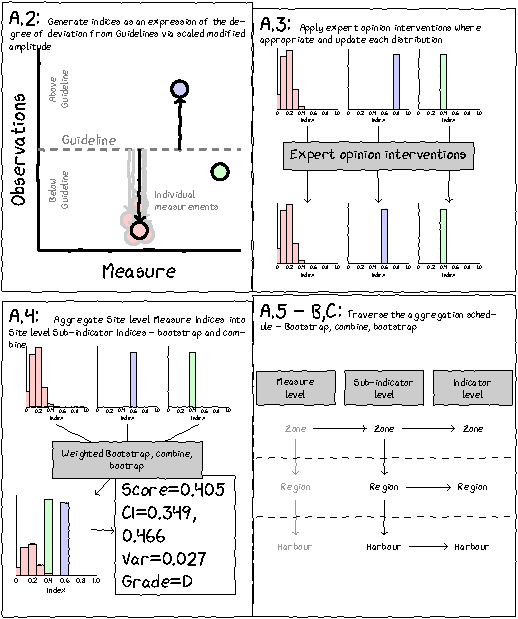
\includegraphics[keepaspectratio]{manual_files/figure-pdf/fig-schematic-1.pdf}}

}

\caption{\label{fig-schematic}Schematic illustrating the major steps of
the Darwin Harbour Report Card. In this fabricated example, there are
three Measures (Red, Green and Blue). Each of the Blue and Green
Measures are represented by a single discrete observation, whereas the
Red Measure is represented by a large collection of observations. Expert
option intervened to lower the blue Measure distribution from observed
values at 0.8 to 0.6.}

\end{figure}%

\subsection{Temporal changes}\label{temporal-changes}

A key goal of any monitoring program is to be able to report on status
and trends. The above methodologies provide the tools for reporting on
the status in any given year. What is also required is the ability to
compare the status between years - that is to report on the changes in
status over time.

The bootstrapp aggregations yield full empirical distributions for each
Measure/Space unit per year. Typically we summarise these distributions
via a mean and confidence interval to simplify their presentation. Then,
if we simply wanted to calculate the change in a score between two
years, we could simply subtract the mean of one year from the other.
However, doing so would loose the information we had on uncertainty. If
on the other hand, we subtracted the distribution for one year from that
of another year, we would obtain a distribution of change values from
which we could provide summaries like mean and confidence intervals.

Since each of the values in the distributions are produced via
bootstrapping, they are not in any specific order (that is they are not
ranked from lowest to highest value) and there are the same number
(\(n\)) of bootstrapp samples in each distribution. Hence, if we line up
the values of two distributions side by side, we can calculate the
difference between each pair of values down the line. This will yield
\(n\) differences. Collectively, these \(n\) differences now represent
the distribution of change values.

In addition to summarising the distribution of change by properties such
as mean and confidence interval, we can also estimate the probability
that the change exceeds a certain value (typically zero). This
calculation is simply the number of values that exceed (zero) divided by
the total number of values and hereafter will be referred to as an
exceedance probability (\(P_E\)).

Between two particular years, scores might generally increase, decrease
or stay the same. To explore an increase, we would report on the
probability that the change values were positive (\(P_E>0\)) and to
report on a decline we would focus on the probability that the change
values were negative (\(P_E<0\)). Note, we cannot report on the
probability that the change values are zero (logically this is
infinitely small). Herein, these exceedance probabilities are
interpreted according to:

\begin{itemize}
\tightlist
\item
  \(P_E \ge 0.95\): strong evidence of change
\item
  \(P_E \ge 0.90\): evidence of change
\item
  \(P_E \ge 0.85\): weak evidence of change
\item
  \(P_E < 0.85\): no evidence of change
\end{itemize}

Within this application, change is explored two ways:

\begin{enumerate}
\def\labelenumi{\arabic{enumi}.}
\tightlist
\item
  annual change - the change between each successive pairs of years
  (e.g.~2016 vs 2017, 2017 vs 2018, etc).
\item
  quinquennial (half-decadal) change - the change between each pair of
  five year blocks of time. This is calculated by first aggregating
  together the blocks of years into single distributions before
  subtracting those distributions.
\end{enumerate}

These changes can then by presented graphically and in tabular form.

\section{Analysis stages}\label{analysis-stages}

\subsection{Stage 2 - obtaining the
data}\label{stage-2---obtaining-the-data}

At the completion of this stage, the Data sidebar menu and Stage 3 \& 4
button will become active and the Data page will be populated with the
raw data and be available for review.

\subsubsection{Read water quality guidelines
data}\label{read-water-quality-guidelines-data}

This task will read in the water quality guidelines information from
the\\
\texttt{../parameters/water\_quality\_guidelines.csv} file.

\subsubsection{Read input data}\label{read-input-data}

This task will sequentially read in each of the water quality data files
from \texttt{../input/}. These files are in the format of
\texttt{\textless{}number\textgreater{}\_wq.csv}, where
\texttt{\textless{}number\textgreater{}} is a two digit number
representation of the sampling year.

\subsubsection{Read in overwrites data}\label{read-in-overwrites-data}

This task will read in each of the overwrites file from
\texttt{../input/overwrites.csv}. The purpose of overwrites is to
provide a mechanism for expert elicitation, whereby grades can be
overwritten in the event that the expert strongly believes that the
observed data are a poor reflection of the genuine health of the
sampling unit.

\subsubsection{Read in the weights data}\label{read-in-the-weights-data}

There are two tasks to read read in the measures weights file from
\texttt{../input/weights\_m.csv} and the spatial weights file from
\texttt{../input/weights\_s.csv}. These files provide a mechanism to
control how much weight different items have in an aggregation. If no
weights are given, then all items are equally weighted during
aggregation.

\subsubsection{Read in aggregation hierarchy
data}\label{read-in-aggregation-hierarchy-data}

This task will read in the aggregation hierarchy file from
\texttt{../input/hierarchy.csv}. The aggregation hierarchy determines
the child items for each aggregation.

\subsubsection{Read in the spatial settings
data}\label{read-in-the-spatial-settings-data}

This task will read in the spatial settings file from
\texttt{../parameters/spatial.csv}. These data form a lookup that relate
zone and area numbers to their names and provides some settings for the
location and colour of labels on maps.

\subsubsection{Validate input data}\label{validate-input-data}

This task performs data validation in accordance with the rules set out
in the following section.

\paragraph{Data requirements}\label{sec-data-requirements}

To be valid, input data must be flat text files (*.csv) comprising:

\begin{itemize}
\item
  \texttt{../input/*\_wq.csv}

  \begin{longtable}[]{@{}
    >{\raggedright\arraybackslash}p{(\linewidth - 4\tabcolsep) * \real{0.1901}}
    >{\raggedright\arraybackslash}p{(\linewidth - 4\tabcolsep) * \real{0.3388}}
    >{\raggedright\arraybackslash}p{(\linewidth - 4\tabcolsep) * \real{0.4711}}@{}}
  \toprule\noalign{}
  \begin{minipage}[b]{\linewidth}\raggedright
  Field
  \end{minipage} & \begin{minipage}[b]{\linewidth}\raggedright
  Description
  \end{minipage} & \begin{minipage}[b]{\linewidth}\raggedright
  Validation conditions
  \end{minipage} \\
  \midrule\noalign{}
  \endhead
  \bottomrule\noalign{}
  \endlastfoot
  Zone & Spatial zone & must be numeric or factor \\
  Region & Spatial region & must be numeric or factor \\
  Source & Source of samples (CFM or Discrete) & must be character or
  factor of either (CFM or Discrete) \\
  Date & Sample data & must be a valid string \\
  Latitude & Latitude of sample & must be a numeric of format -d.d \\
  Longitude & Longitude of sample & must be a numeric of format d.d \\
  Chla\_mug\_PER\_L & Chlorophyll-a concentration & must contain only
  numbers or start with a `\textless{}' symbol \\
  Turbidity\_NTU & Turbidity concentration & must contain only numbers
  or start with a `\textless{}' symbol \\
  Turbidity\_NTU & & should not exist for Discrete source \\
  DO\_PERCENT\_saturation & Percentage dissolved oxygen & must contain
  only numbers or start with a `\textless{}' symbol \\
  NH3\_mug\_PER\_L & Ammonium concentration & must contain only numbers
  or start with a `\textless{}' symbol \\
  NH3\_mug\_PER\_L & & should not exist for CFM source \\
  PO4\_mug\_PER\_L & Phosphate concentration & must contain only numbers
  or start with a `\textless{}' symbol \\
  PO4\_mug\_PER\_L & & should not exist for CFM source \\
  Nox\_mug\_PER\_L & Nox (nitrate and nitrite) concentration & must
  contain only numbers or start with a `\textless{}' symbol \\
  Nox\_mug\_PER\_L & & should not exist for CFM source \\
  \end{longtable}
\item
  \texttt{../input/hierarchy.csv}

  \begin{longtable}[]{@{}
    >{\raggedright\arraybackslash}p{(\linewidth - 4\tabcolsep) * \real{0.1000}}
    >{\raggedright\arraybackslash}p{(\linewidth - 4\tabcolsep) * \real{0.5000}}
    >{\raggedright\arraybackslash}p{(\linewidth - 4\tabcolsep) * \real{0.4000}}@{}}
  \toprule\noalign{}
  \begin{minipage}[b]{\linewidth}\raggedright
  Field
  \end{minipage} & \begin{minipage}[b]{\linewidth}\raggedright
  Description
  \end{minipage} & \begin{minipage}[b]{\linewidth}\raggedright
  Validation conditions
  \end{minipage} \\
  \midrule\noalign{}
  \endhead
  \bottomrule\noalign{}
  \endlastfoot
  Component & Highest level of measure hierarchy (always Environmental)
  & must contain characters \\
  IndicatorGroup & Next measure level (always Water Quality) & must
  contain characters \\
  Indicator & Next measure level (always Water Quality) & must contain
  characters \\
  Subindicator & Either Nutrients or Physico-chem & must contain
  characters \\
  Measure & Name of the Measure & must contain characters \\
  \end{longtable}
\item
  \texttt{../input/weights\_*.csv}

  \begin{longtable}[]{@{}
    >{\raggedright\arraybackslash}p{(\linewidth - 4\tabcolsep) * \real{0.1569}}
    >{\raggedright\arraybackslash}p{(\linewidth - 4\tabcolsep) * \real{0.5784}}
    >{\raggedright\arraybackslash}p{(\linewidth - 4\tabcolsep) * \real{0.2647}}@{}}
  \toprule\noalign{}
  \begin{minipage}[b]{\linewidth}\raggedright
  Field
  \end{minipage} & \begin{minipage}[b]{\linewidth}\raggedright
  Description
  \end{minipage} & \begin{minipage}[b]{\linewidth}\raggedright
  Validation conditions
  \end{minipage} \\
  \midrule\noalign{}
  \endhead
  \bottomrule\noalign{}
  \endlastfoot
  Component & Highest level of measure hierarchy (always Environmental)
  & must contain characters \\
  IndicatorGroup & Next measure level (always Water Quality) & must
  contain characters \\
  Indicator & Next measure level (always Water Quality) & must contain
  characters \\
  Subindicator & Either Nutrients or Physico-chem & must contain
  characters \\
  Measure & Name of the Measure & must contain characters \\
  Zone & Spatial zone & must be numeric or factor \\
  Region & Spatial region & must be numeric or factor \\
  Site & Spatial site & must be numeric or factor \\
  Weight & Spatial site & must be numeric \\
  \end{longtable}

  \begin{description}
  \tightlist
  \item[Could be empty]
  \{tbl-colwidths=``{[}25,35,40{]}''\}
  \end{description}
\item
  \texttt{../input/overwrites.csv}

  \begin{longtable}[]{@{}
    >{\raggedright\arraybackslash}p{(\linewidth - 4\tabcolsep) * \real{0.1343}}
    >{\raggedright\arraybackslash}p{(\linewidth - 4\tabcolsep) * \real{0.4403}}
    >{\raggedright\arraybackslash}p{(\linewidth - 4\tabcolsep) * \real{0.4254}}@{}}
  \toprule\noalign{}
  \begin{minipage}[b]{\linewidth}\raggedright
  Field
  \end{minipage} & \begin{minipage}[b]{\linewidth}\raggedright
  Description
  \end{minipage} & \begin{minipage}[b]{\linewidth}\raggedright
  Validation conditions
  \end{minipage} \\
  \midrule\noalign{}
  \endhead
  \bottomrule\noalign{}
  \endlastfoot
  Component & Highest level of measure hierarchy (always Environmental)
  & must contain characters \\
  IndicatorGroup & Next measure level (always Water Quality) & must
  contain characters \\
  Indicator & Next measure level (always Water Quality) & must contain
  characters \\
  Subindicator & Either Nutrients or Physico-chem & must contain
  characters \\
  Measure & Name of the Measure & must contain characters \\
  Source & Source of samples (CFM or Discrete) & must be character or
  factor of either (CFM or Discrete) \\
  Region & Spatial region & must be numeric or factor \\
  Zone & Spatial zone & must be numeric or factor \\
  Site & Spatial site & must be numeric or factor \\
  overwrittenGrade & Grade to apply (overwrite observations) & must
  contain characters (A, B, C, D or E) \\
  \end{longtable}

  \begin{description}
  \tightlist
  \item[Could be empty]
  \{tbl-colwidths=``{[}25,35,40{]}''\}
  \end{description}
\item
  \texttt{../parameters/water\_quality\_guidelines.csv}

  \begin{longtable}[]{@{}
    >{\raggedright\arraybackslash}p{(\linewidth - 4\tabcolsep) * \real{0.2500}}
    >{\raggedright\arraybackslash}p{(\linewidth - 4\tabcolsep) * \real{0.3500}}
    >{\raggedright\arraybackslash}p{(\linewidth - 4\tabcolsep) * \real{0.4000}}@{}}
  \toprule\noalign{}
  \begin{minipage}[b]{\linewidth}\raggedright
  Field
  \end{minipage} & \begin{minipage}[b]{\linewidth}\raggedright
  Description
  \end{minipage} & \begin{minipage}[b]{\linewidth}\raggedright
  Validation conditions
  \end{minipage} \\
  \midrule\noalign{}
  \endhead
  \bottomrule\noalign{}
  \endlastfoot
  ZoneName & Zone name & must contain characters \\
  HydstraName & Name in hydstra & must contain characters \\
  Conversion & Unit conversion factor & must be numeric \\
  Measure & Name of the Measure & must contain characters \\
  UnitsLabel & Name of the Measure including units & must contain
  characters \\
  Label & Name of the Measure including units (formatted for LaTeX) &
  must contain characters \\
  DirectionOfFailure & Direction of failure relative to guideline value
  & must be a single character (B or H) \\
  GL & Water quality guideline value & must contain only numbers or
  start with a `\textless{}' symbol \\
  RangeFrom & Water quality guideline lower limit of range (for DO) &
  must contain only numbers or start with a `\textless{}' symbol \\
  RangeTo & Water quality guideline upper limit of range range (for DO)
  & must contain only numbers or start with a `\textless{}' symbol \\
  DetectionLimit & Limit of detection value & must contain only numbers
  or start with a `\textless{}' symbol \\
  \end{longtable}
\item
  \texttt{../parameters/spatial.csv}

  \begin{longtable}[]{@{}
    >{\raggedright\arraybackslash}p{(\linewidth - 4\tabcolsep) * \real{0.2500}}
    >{\raggedright\arraybackslash}p{(\linewidth - 4\tabcolsep) * \real{0.3500}}
    >{\raggedright\arraybackslash}p{(\linewidth - 4\tabcolsep) * \real{0.4000}}@{}}
  \toprule\noalign{}
  \begin{minipage}[b]{\linewidth}\raggedright
  Field
  \end{minipage} & \begin{minipage}[b]{\linewidth}\raggedright
  Description
  \end{minipage} & \begin{minipage}[b]{\linewidth}\raggedright
  Validation conditions
  \end{minipage} \\
  \midrule\noalign{}
  \endhead
  \bottomrule\noalign{}
  \endlastfoot
  Region & Spatial region & must be numeric or factor \\
  RegionName & Region name & must contain characters \\
  Zone & Spatial zone & must be numeric or factor \\
  ZoneName & Zone name & must contain characters \\
  Lab\_lat & Latitude of zone label on maps & must be a numeric of
  format -d.d \\
  Lab\_long & Longitude of zone label on maps & must be a numeric of
  format d.d \\
  HexColor & Hexidecimal colour code for zone labels on maps & must be a
  six digit hex code proceeded by a `\#' \\
  \end{longtable}
\end{itemize}

\subsection{Stage 3 - Prepare spatial
data}\label{stage-3---prepare-spatial-data}

\subsubsection{Read in shapefiles}\label{read-in-shapefiles}

This task will read in individual shapefiles from
\texttt{../parameters/GIS}. The files are: - \texttt{RCZ\_rev24.shp} -
\texttt{SBZone\_upper.shp} - \texttt{Middle\_Harbour\_Upper.shp}

\subsubsection{Combine shapefiles}\label{combine-shapefiles}

This task will combine all shapefiles into a single shapefile

\subsection{Stage 4 - processing the
data}\label{stage-4---processing-the-data}

\subsubsection{Combine water quality
data}\label{combine-water-quality-data}

The water quality data are read in as separate csv files. Although
technically they could have been consolidated into a single file before
opening this application, maintaining separate files for each year does
allow the user to isolate any validation issues to a single year
(thereby making them easier to located and correct).

The current task will combine all the water quality data into a single
data set.

\subsubsection{Process dates}\label{process-dates}

Spreadsheets often display dates in different formats from what they
actually store internally and what they export. It is always advisable
when exporting dates from spreadsheets to export them as strings (words)
rather than numbers (number of seconds past a reference date) as these
are typically less ambiguous.

The current task will process the dates from strings into genuine date
objects

\subsubsection{Filter the date range of the
data}\label{filter-the-date-range-of-the-data}

It is possible to restrict the analyses to a narrower range of dates
than those that appear in the observed data. For example, the observed
data might include some samples from an otherwise incomplete sampling
year, and it might be desirable to exclude these samples. Hence, this
task determines whether a \texttt{start\_date} or \texttt{end\_date}
have been defined in \texttt{../parameters/config.ini} and if so, uses
them to trim the temporal range of the data.

The tables within the \textbf{Processed data} tab of the \textbf{Data}
page will also be populated and the \texttt{Data} page will be available
for review.

\subsubsection{Select Measures}\label{select-measures}

In order to compute indices, it is necessary to compare observed values
to associated guideline values. In the current context a
\textbf{Measure} is an observable property of water quality (such as
Chlorophyl-a, Turbidity, Nox etc) - it is the analyte that is measured.
This current task will exclude any measures for which there are no
guideline values as these cannot be analysed further.

\subsubsection{Define the focal year}\label{define-the-focal-year}

The \textbf{focal year} represents the year that will be considered the
focal sampling year for the analyses. All outputs will be stored in a
folder reflecting this display diagnostics for this the focal year is
the most recent sampling year. Furthermore, many of the QAQC diagnostics
pertain specifically to this focal year alone.

\subsubsection{Pivot data into longer
format}\label{pivot-data-into-longer-format}

Although it is often convenient to transcribe and store data in
\emph{wide} format (one in which each measure has its own column and
each row represents a single sample collection), this format is
illsuited for analyses and graphics in R. Analyses and graphics prefer
data to be in \emph{long} format. The following two tables highlight the
differences between wide (top table) and long (bottom table) formats:

\begin{longtable}[]{@{}
  >{\raggedright\arraybackslash}p{(\linewidth - 10\tabcolsep) * \real{0.0811}}
  >{\raggedright\arraybackslash}p{(\linewidth - 10\tabcolsep) * \real{0.1622}}
  >{\raggedright\arraybackslash}p{(\linewidth - 10\tabcolsep) * \real{0.1351}}
  >{\raggedright\arraybackslash}p{(\linewidth - 10\tabcolsep) * \real{0.2162}}
  >{\raggedright\arraybackslash}p{(\linewidth - 10\tabcolsep) * \real{0.2027}}
  >{\raggedright\arraybackslash}p{(\linewidth - 10\tabcolsep) * \real{0.2027}}@{}}
\toprule\noalign{}
\begin{minipage}[b]{\linewidth}\raggedright
Zone
\end{minipage} & \begin{minipage}[b]{\linewidth}\raggedright
Date
\end{minipage} & \begin{minipage}[b]{\linewidth}\raggedright
Source
\end{minipage} & \begin{minipage}[b]{\linewidth}\raggedright
Chla\_mug\_PER\_L
\end{minipage} & \begin{minipage}[b]{\linewidth}\raggedright
Turbidity\_NTU
\end{minipage} & \begin{minipage}[b]{\linewidth}\raggedright
Nox\_mug\_PER\_L
\end{minipage} \\
\midrule\noalign{}
\endhead
\bottomrule\noalign{}
\endlastfoot
1 & 01/06/2016 & CFM & 1.338 & 2.68 & NA \\
1 & 01/06/2016 & CFM & 1.376 & 2.63 & NA \\
1 & 02/06/2016 & Discrete & 0.279 & NA & 0.013 \\
1 & 02/06/2016 & Discrete & 0.178 & NA & 0.017 \\
\end{longtable}

\begin{longtable}[]{@{}lllll@{}}
\toprule\noalign{}
Zone & Date & Source & Measure & Value \\
\midrule\noalign{}
\endhead
\bottomrule\noalign{}
\endlastfoot
1 & 01/06/2016 & CFM & Chla\_mug\_PER\_L & 1.338 \\
1 & 01/06/2016 & CFM & Chla\_mug\_PER\_L & 1.376 \\
1 & 02/06/2016 & Discrete & Chla\_mug\_PER\_L & 0.279 \\
1 & 02/06/2016 & Discrete & Chla\_mug\_PER\_L & 0.178 \\
1 & 01/06/2016 & CFM & Turbidity\_NTU & 2.68 \\
1 & 01/06/2016 & CFM & Turbidity\_NTU & 2.63 \\
1 & 02/06/2016 & Discrete & Turbidity\_NTU & NA \\
1 & 02/06/2016 & Discrete & Turbidity\_NTU & NA \\
1 & 01/06/2016 & CFM & Nox\_mug\_PER\_L & NA \\
1 & 01/06/2016 & CFM & Nox\_mug\_PER\_L & NA \\
1 & 02/06/2016 & Discrete & Nox\_mug\_PER\_L & 0.013 \\
1 & 02/06/2016 & Discrete & Nox\_mug\_PER\_L & 0.017 \\
\end{longtable}

This task will therefore pivot the data from wide to long format.

\subsubsection{Join the guidelines data to the water quality
data}\label{join-the-guidelines-data-to-the-water-quality-data}

This task will join (merge) the guideline data with the water quality
data based on the Zones.

\subsubsection{Apply spatial
information}\label{apply-spatial-information}

This task will use the shapefiles to assign spatial information (Zones
and Regions) based on the latitude and longitude of the samples.

\subsubsection{Make spatial lookup}\label{make-spatial-lookup}

This stage creates a lookup table that relates each of the spatial
scales to one another. This lookup is used to inject the spatial
information into the data and modelled derivatives after they are
created and in so doing prevents the need to spatially join the data
each time it is required.

\subsubsection{Apply unit conversions}\label{apply-unit-conversions}

In addition to defining the guideline values, the
\texttt{../input/water\_quality\_guidelines.csv} file defines any unit
conversions that need to be applied. This task applies those unit
conversions.

\subsubsection{Apply limit of detection
rules}\label{apply-limit-of-detection-rules}

This task applies limit of detection rules. Specifically, for all
measures other than dissolved oxygen, if the observed value is below the
detection limit, then the observed value is replaced by the detection
limit. In the case of dissolved oxygen, if the observed value is less
than 50, the observed value is replaced by NA (a missing value). In
either case, a flag is added if a limit of detection replacement is
made.

\subsubsection{Join the aggregation
hierarchy}\label{join-the-aggregation-hierarchy}

The aggregation hierarchy determines what items are aggregated together
during the bootstrapp aggregation process. This task joins the
aggregation schedule into the data.

\subsection{Stage 5 - Calculate
indices}\label{stage-5---calculate-indices}

\subsubsection{Load the data}\label{load-the-data}

This task loads the processed data in preparation for indice
calculations.

\subsubsection{Calculate indices}\label{calculate-indices}

\subsubsection{Prepare for
bootstrapping}\label{prepare-for-bootstrapping}

This current step prepares the Site/Year/Source level data for
bootstrapp aggregation by repeatedly sampling these data (according to
the nominated number of bootstrapp samples, \(n\), set in the
\texttt{../parameters/config.ini} file). In the case that only a single
observation was collected at a specific site in a specific year for a
specific source, then this observation will be repeated \(n\) times.

\subsection{Stage 6 - QAQC}\label{stage-6---qaqc}

\subsection{Stage 7 - Bootstrapping}\label{stage-7---bootstrapping}

\subsubsection{Load data}\label{load-data}

This task will load the processed data.

\subsubsection{Load the indices}\label{load-the-indices}

This task will load the indices ready for bootstrapping.

\subsubsection{Process the overwrites}\label{process-the-overwrites}

This task will determine what overwrites have been defined in the
\texttt{../input/overwrites.csv} file and make those specific changes to
the indices prior to bootstrapping. Essentially, this task involves
replacing the indices and grades calculated in Stage 5 (for the
nominated measure/spatial scale) with those nominated the overwrites.

\subsubsection{Process the weights}\label{process-the-weights}

This task will determine what weights (measure or spatial) have been
defined in \texttt{../input/weights\_m.csv} and
\texttt{../input/weights\_s.csv} respectively and prepare for applying
these weights during the appropriate aggregation phase.

\subsubsection{Series of aggregations}\label{series-of-aggregations}

There will then be a series of tasks that perform each of the
hierarchical bootstrapp aggregations outlined in Figure~\ref{fig-hier}.

\subsection{Stage 8 - Summaries}\label{stage-8---summaries}

This stage will generate a series of summary plots in the form of
temporal trend plots and effects plots. At the end of this stage, the
\emph{Summaries} page will be enabled for review.

\subsubsection{Load the data}\label{load-the-data-1}

This task will load the processed data.

\subsubsection{Compile the scores}\label{compile-the-scores}

During the hierarchical boostrapp aggregation process, each
Measure/Space combination is stored as its own data artifact. The
current task will read each of these in an compile them together into a
single object.

\subsubsection{Series of trend plots}\label{series-of-trend-plots}

For each of the Measure/Space combinations, a temporal trend figure will
be produced.

\subsubsection{Calculate effects}\label{calculate-effects}

This task will loop through each Measure/Space combination and calculate
the annual and quinquennial (half-decadal) changes.

\subsection{Effects plots}\label{effects-plots}

This task will generate effects plots for each Measure/Space/Change
combination.

\section{Application pages}\label{application-pages}

\subsection{Landing page}\label{sec-landing}

To run this tool, please adhere to the following steps:

\begin{enumerate}
\def\labelenumi{\arabic{enumi}.}
\tightlist
\item
  review the \emph{Path Settings} (specifically checking the
  \textbf{``Data input dir''}) and ensuring that there is at least one
  data file listed in the box under this setting
\item
  review the \emph{Run Settings}. In particular,

  \begin{itemize}
  \tightlist
  \item
    consider whether you need to \textbf{Clear the previous data} -
    clicking the button to do so. Clearing the previous data deletes all
    cache and ensure that the analyses are performed fresh. \textbf{This
    is recommended whenever the input data changes}. Not clearing the
    previous data allows the user to skip directly to later run stages
    if earlier stages have already been run.
  \end{itemize}
\item
  navigate the \emph{Dashboard} via the menu on the left sidebar
\end{enumerate}

In the \emph{Run settings} panel, there is a \textbf{Run in sequence}
toggle. By default, this toggle is set to ``Yes'' which ensures that all
stages must be run in sequence and the various pages will become active
once the appropriate stages have been complete. Toggling this switch to
``NO'' will instantly make all side menus, pages and run buttons become
available. The purpose of this is to allow the user to re-visit the
outcomes of analyses without the need to completely re-run the entire
analysis. This is particularly useful if the user is returning to the
analyses at a later date.

\begin{tcolorbox}[enhanced jigsaw, left=2mm, colback=white, leftrule=.75mm, breakable, colframe=quarto-callout-color-frame, arc=.35mm, toprule=.15mm, opacityback=0, rightrule=.15mm, bottomrule=.15mm]

Note

Toggling the \textbf{Run in sequence} switch to ``No'' assumes that
numerous artifacts (data saved throughtout the analysis process) are
available and thus should only be considered after the analyses have
been run through completely at some time. Never toggle this switch
straight after clicking the ``Clear previous data'' button.

\end{tcolorbox}

\subsection{Dashboard}\label{sec-dashboard}

The analysis pipeline comprises numerous \textbf{Stages}, each of which
is made up of several more specific \textbf{Tasks}. The individual Tasks
represent an action performed in furtherance of the analysis and of
which there are reportable diagnostics. For example, once the
application loads, the first Stage of the pipeline is to prepare the
environment. The first Task in this Stage is to load the necessary R
packages used by the codebase. Whilst technically, this action consists
of numerous R calls (one for each package that needs to be loaded), the
block of actions are evaluated as a set.

Initially, all upcoming tasks are reported as ``pending'' ({}). As the
pipeline progresses, each Task is evaluated and a status is returned as
either ``success'' ({}) or ``failure'' ({}).

The Stage that is currently (or most recently) being run will be
expanded, whereas all other Stages will be collapsed (unless they
contain errors). It is also possible to expand/collapse a Stage by
double clicking on its title (or the small arrow symbol at the left side
of the tree).

As the pipeline progresses, Task logs are written to a log file and
echoed to the \textbf{Logs} panel. Each row represents the returned
status of a specific Task and are formatted as:

\begin{itemize}
\tightlist
\item
  the time/date that the Task was evaluated
\item
  the Task status, which can be one of:

  \begin{itemize}
  \tightlist
  \item
    \texttt{SUCCESS} the task succeeded
  \item
    \texttt{FAILURE} the task failed and should be investigated
  \item
    \texttt{WARNING} the task contained a warning - typically these can
    be ignored as they are usually passed on from underlying routines
    and are more targetted to developers than users.
  \end{itemize}
\item
  the Stage followed by the Task name
\item
  in the case of errors and warnings, there will also be the error or
  warning message passed on from the underlying routines. These can be
  useful for helping to diagnose the source and cause of issues.
\end{itemize}

The Logs in the Log panel are presented in chronological order and will
autoscroll such that the most recent log is at the bottom of the
display. If the number of Log lines exceeds 10, a scroll bar will appear
on the right side of the panel to help reviewing earlier Logs.

\begin{tcolorbox}[enhanced jigsaw, left=2mm, colback=white, leftrule=.75mm, breakable, colframe=quarto-callout-color-frame, arc=.35mm, toprule=.15mm, opacityback=0, rightrule=.15mm, bottomrule=.15mm]

Note

The Status and Logs are completely refreshed each time the application
is restarted.

\end{tcolorbox}

The Progress panel also has a tab (called \textbf{Terminal-like}) which
provides an alternative representation of the status and progress of the
pipeline.

\subsection{Data}\label{sec-data}

The Data page comprises two panels or subpages accessable by tabs named
``Raw data'' and ``Processed data'' at the top of the page.

\begin{tcolorbox}[enhanced jigsaw, left=2mm, leftrule=.75mm, bottomrule=.15mm, toptitle=1mm, colbacktitle=quarto-callout-note-color!10!white, bottomtitle=1mm, arc=.35mm, colback=white, breakable, opacitybacktitle=0.6, coltitle=black, colframe=quarto-callout-note-color-frame, titlerule=0mm, toprule=.15mm, opacityback=0, title=\textcolor{quarto-callout-note-color}{\faInfo}\hspace{0.5em}{Note}, rightrule=.15mm]

The contents of the Processed data subpage will not be revealed until
the completion of Stage 3.

\end{tcolorbox}

\subsubsection{Raw data panel}\label{raw-data-panel}

The \textbf{Raw data} panel displays the input data and associated
validation summaries (once the data have been loaded - that is, once
Stage 2 has been complete). The table (main metadata table) above
initially has a row for each of the input files.

The title of each input file name is displayed in the first column
(\textbf{File}). The size and file creation time in the next two columns
(fields). The \textbf{Status} field indicates whether the data in the
various files are considered valid ({}) or not ({}).

Clicking anywhere in a row containing will select the row and once a row
is selected, information in both the \emph{Data} and \emph{Validation
issues} tabs will be populated.

Initially, the \emph{Instructions} tab will be active and visible
(providing these instructions). The other two tabs are:

\begin{itemize}
\item
  \textbf{Data}: provides a view of the data beyind the selected row in
  the main metadata table and a mechanism to download those data. Only
  the first 10 rows are displayed in the table, the others being
  accessable via the controls under the table.

  Note, all numerical values are displayed only to three decimal places,
  yet the actual underlying data is full resolution.
\item
  \textbf{Validation issues}: highlights and displays a description any
  validation issues associated with the selected row in the main
  metadata table.

  If there were no validation issues, this table will be empty.
  Otherwise, the description field will indicate the nature of the
  violation and in the case of issues with an individual record, the
  offending row will be presented across the remaining cells in the row.
  For more information about the validation tests, please refer to the
  \textbf{Data requirements} box (to the right of this box in the app).
\end{itemize}

Underneath both the Data and Validation tables, there is a
\textbf{Download as csv} button. Via this button, you can download a
comma separated text file version of the data in the table for further
review in a spreadsheet of your choice. Once you click this button, you
will be prompted to navigate to a suitable location to store the file.

\subsubsection{Processed data panel}\label{processed-data-panel}

The Processed data panel displays the first 10 rows of the complete,
compiled and processed data set. Descriptions of each field of these
data are provided in the table below.

\begin{tcolorbox}[enhanced jigsaw, left=2mm, leftrule=.75mm, bottomrule=.15mm, toptitle=1mm, colbacktitle=quarto-callout-note-color!10!white, bottomtitle=1mm, arc=.35mm, colback=white, breakable, opacitybacktitle=0.6, coltitle=black, colframe=quarto-callout-note-color-frame, titlerule=0mm, toprule=.15mm, opacityback=0, title=\textcolor{quarto-callout-note-color}{\faInfo}\hspace{0.5em}{Note}, rightrule=.15mm]

This panel will not become active until the completion of Stage 3.

\end{tcolorbox}

The \textbf{Processed data} panel displays the processed data. As part
of the processing, the following new fields will be created:

\begin{longtable}[]{@{}
  >{\raggedright\arraybackslash}p{(\linewidth - 2\tabcolsep) * \real{0.2000}}
  >{\raggedright\arraybackslash}p{(\linewidth - 2\tabcolsep) * \real{0.8000}}@{}}
\toprule\noalign{}
\begin{minipage}[b]{\linewidth}\raggedright
Field
\end{minipage} & \begin{minipage}[b]{\linewidth}\raggedright
Description
\end{minipage} \\
\midrule\noalign{}
\endhead
\bottomrule\noalign{}
\endlastfoot
Source & Source of samples (CFM or Discrete) \\
Date & Sample data \\
Latidude & Latitude of sample \\
Longitude & Longitude of sample \\
Focal\_Year & Year in which analyses are logged (typically the most
recent year) \\
Year & Year of sample \\
Measure & Name of the Measure \\
Value & Observed measure value \\
OldZone & Old Zone name \\
Region & Darwin Harbour Region number \\
Zone & Darwin Harbour Zone number \\
ZoneName & Name of the Darwin Harbour Zone \\
HydstraName & Name of the measure in hydstra \\
Conversion & Unit conversion factor \\
UnitsLabel & Name of the Measure including units \\
Label & Name of the Measure including units (in LaTeX format) \\
DirectionOfFailure & Direction of failure relative to guideline value \\
GL & Water quality guideline value \\
RangeFrom & Water quality guideline lower limit of range (for DO) \\
RangeTo & Water quality guideline upper limit of range range (for DO) \\
DetectionLimit & Limit of detection value \\
Flag & Limit of detection flag (when limit of detection applied) \\
Component & Highest level of measure hierarchy (always Environmental) \\
IndicatorGroup & Next measure level (always Water Quality) \\
Indicator & Next measure level (always Water Quality) \\
Subindicator & Either Nutrients or Physico-chem \\
\end{longtable}

Under the column (field) headings in the Processed data panel table,
there are input boxes that act as filters. The data presented in the
table will be refined to just those cases that match the input string as
it is being typed. It is possible to engage with any or all of these
filters to help refine the search.

Under the table there is a \textbf{Download as csv} button. Via this
button, you can download a comma separated text file version of the data
in the table for further review in a spreadsheet of your choice. Once
you click this button, you will be prompted to navigate to a suitable
location to store the file.

\subsection{QAQC}\label{qaqc}

The QAQC page comprises two panels or subpages accessable by tabs at the
top of the page and named ``Observations'' and ``Boxplots''.

\subsubsection{Observations}\label{observations}

This page displays multi-panel figures depicting the observed data for a
selected year conditional on Measures (columns) and Zones (rows). These
figures at organised according to three \emph{Source} types (all, CFM
and Discrete) and these are activated via three large tab buttons down
the left side of the panel. The sampling year is selected via a dropdown
box in a panel above the figures.

The individual figures depict the observed Measures (columns) of all
Water Quality data from each of eleven Zones (rows). The red vertical
line indicates associated Water Quality Guideline value. The transparent
red band indicates a range of values represented by half and twice the
guideline value (equivalent to the Scaled Modified Amplitude index
capping domain). The blue band represents the Guideline range for
Dissolved Oxygen. Note, the y-axis only represents jittered and
unordered space. temporal sampling design.

\subsubsection{Boxplots}\label{boxplots}

This page displays multi-panel figures depicting boxplots for the
observed data for a selected year conditional on Measures (columns) and
Zones (x-axes).

These figures at organised according to three types (all, timeseries and
zones) and these are activated via three large tab buttons down the left
side of the panel. The sampling year is selected via a dropdown box in a
panel above the figures.

\begin{itemize}
\tightlist
\item
  all: the figure depicts the boxplots of the observed Measures (panels)
  of Water Quality data from each of eleven Zones (x-axes) for each
  source. The horizontal dashed lines indicate the associated Water
  Quality Guideline values.
\item
  timeseries: the figure depicts the boxplots of the observed Measures
  (panels) of Water Quality data from each of the eleven Zones (x-axes)
  across all sampling years. The horizontal dashed lines indicate the
  associated Water Quality Guideline values.
\item
  zones: the figure depicts the boxplots of the observed Measures
  (panels) of Water Quality data from selected zones for the selected
  sampling year. The dropdown is used to select the zones. The
  horizontal dashed lines indicate the associated Water Quality
  Guideline values.
\end{itemize}

\subsection{Summaries}\label{summaries}

The Summaries page comprises a horizontal selector panel along with
three three panels or subpages accessable by tabs at the tabs and named
``Trends'', ``Annual effects'' and ``Contrast effects''.

Within the selector panel, there are a series of dropdown selection
boxes for choosing between a set of candidates for each of the
following:

\begin{itemize}
\tightlist
\item
  Subindicator
\item
  Measure
\item
  Region
\item
  Zone
\item
  Source
\end{itemize}

In each case, in addition to candidates created from the unique values
observed in the data, there is also an ``All'' candidate. The All
candidate represents the aggregation of the other candidates. For
example, the All \emph{Region} candidate allows for the selection of the
Whole of Harbour. Similarly, the All candidate in the \emph{Measures}
selector when the \emph{Subindicator} selector has the ``Physico-chem''
candidate selected indicates the aggregate of all Measures across
Physico-chem.

The selectors are linked such that selecting a candidate from one
dropdown (e.g.~\emph{Region}) will determine what candidates are
available in other selector dropdowns (e.g.~\emph{Zones} and
\emph{Source}). By default, the All candidate is selected for all
selectors. This equates to the Whole of Harbour Indicator scores
(i.e.~the highest level of aggregation).

\subsubsection{Trends}\label{trends}

The trend plots display the temporal trend in indicator scores.
Uncertainty (95\% confidence intervals) in the scores are depicted by
vertical whiskers and the open symbols are coloured according to the
grade associated with the mean score. Dashed horizontal lines indicate
the grade boundaries.

\subsubsection{Annual effects}\label{annual-effects}

The distribution of comparisons (absolute change in indicator score) of
each sampling year to the previous sampling year are depicted by density
plots with point and whiskers (mean and 95\% confidence intervals)
below. Exceedance probabilitys for increase (\(P(\Delta>0)\)) and
decrease (\(P(\Delta<0)\)) are overlayed onto the density plots. Density
distributions are coloured according to whether there is strong evidence
for an increase (green) or decrease (red) or no evidence of change
(gray).

\subsubsection{Contrast effects}\label{contrast-effects}

The distribution of comparisons (absolute change in indicator score) of
each half-decade to the previous half-decade are depicted by density
plots with point and whiskers (mean and 95\% confidence intervals)
below. Exceedance probabilitys for increase (\(P(\Delta>0)\)) and
decrease (\(P(\Delta<0)\)) are overlayed onto the density plots. Density
distributions are coloured according to whether there is strong evidence
for an increase (green) or decrease (red) or no evidence of change
(gray).




\end{document}
